\documentclass[a4paper,11pt,oneside]{report}
\usepackage{float}
\usepackage{chngpage}
\usepackage{acro}
\usepackage{subcaption}
\usepackage{minted}
\usepackage{bm}
\usepackage{nameref}
\usepackage{hyperref}
\usepackage{etoolbox}
\usepackage{dirtree}
\usepackage{amsmath}
\usepackage[linesnumbered, ruled, vlined]{algorithm2e}
\usepackage[table,x11names]{xcolor}
\usepackage[english]{./_template/disal_report_template}

% Configuration for `algorithm2e`
\newcommand\mycommfont[1]{\footnotesize\ttfamily\textcolor{blue}{#1}}
\SetCommentSty{mycommfont}

% Configuration for chapter that will be shown
\newtoggle{FULL_REPORT}
\toggletrue{FULL_REPORT}
%\togglefalse{FULL_REPORT}

% Configuration for `acro`
\DeclareAcronym{ros}{
  short = ROS,
  long = Robotic Operating System
}

\DeclareAcronym{ros2}{
  short = \acs{ros}2,
  long = \acl{ros}2
}

\DeclareAcronym{ros1}{
  short = \acs{ros}1,
  long = \acl{ros}1
}

\DeclareAcronym{api}{
  short = API,
  long = Application Programming Interface
}

\DeclareAcronym{urdf}{
  short = URDF,
  long = Unified Robot Description Format
}

\DeclareAcronym{slam}{
  short = SLAM,
  long = Simultaneous Localization And Mapping
}

\DeclareAcronym{epfl}{
  short = EPFL,
  long = École Polytechnique Fédérale de Lausanne
}

\DeclareAcronym{ci}{
  short = CI,
  long = Continuous Integration
}

\DeclareAcronym{cd}{
  short = CD,
  long = Continuous Delivery
}

\DeclareAcronym{cicd}{
  short = \acs{ci}/\acs{cd},
  long = \ac{ci} and \ac{cd}
}

\DeclareAcronym{i2c}{
  short = I\textsuperscript{2}C,
  long = Inter-Integrated Circuit
}

\DeclareAcronym{uart}{
  short = UART,
  long = Universal Asynchronous Receiver-Transmitter
}

\DeclareAcronym{cpu}{
  short = CPU,
  long = Central Processing Unit
}

\DeclareAcronym{mcu}{
  short = MCU,
  long = Microcontroller Unit
}

\DeclareAcronym{tof}{
  short = ToF,
  long = Time of Flight
}

\DeclareAcronym{dds}{
  short = DDS,
  long = Data Distribution Service
}

\DeclareAcronym{udp}{
  short = UDP,
  long = User Datagram Protocol
}

\DeclareAcronym{jpeg}{
  short = JPEG,
  long = Joint Photographic Experts Group
}

\DeclareAcronym{fps}{
  short = FPS,
  long = Frames Per Second
}

\DeclareAcronym{rgb}{
  short = RGB,
  long = Red Green Blue
}

\DeclareAcronym{gpu}{
  short = GPU,
  long = Graphics Processing Unit
}

\DeclareAcronym{os}{
  short = OS,
  long = Operating System
}

\DeclareAcronym{qos}{
  short = QoS,
  long = Quality of Service
}

\DeclareAcronym{fpga}{
  short = FPGA,
  long = Field-Programmable Gate Array
}

\DeclareAcronym{lidar}{
  short = LiDAR,
  long = Light Detection And Ranging sensor
}

\DeclareAcronym{lts}{
  short = LTS,
  long = Long-Term Support 
}

\DeclareAcronym{mips}{
  short = MIPS,
  long = Million Instructions Per Second
}

\DeclareAcronym{dsp}{
  short = DSP,
  long = Digital Signal Processor
}

\DeclareAcronym{fpu}{
  short = FPU,
  long = Floating-Point Unit
}

\DeclareAcronym{dma}{
  short = DMA,
  long = Direct Memory Access 
}

\DeclareAcronym{led}{
  short = LED,
  long = Light-Emitting Diode 
}

\DeclareAcronym{imu}{
  short = IMU,
  long = Inertial Measurement Unit 
}

\DeclareAcronym{pcb}{
  short = PCB,
  long = Printed Circuit Board
}

\DeclareAcronym{pc}{
  short = PC,
  long = Personal Computer
}

\DeclareAcronym{ode}{
  short = ODE,
  long = Open Dynamics Engine
}

\DeclareAcronym{tcp}{
  short = TCP,
  long = Transmission Control Protocol
}

\DeclareAcronym{rgbled}{
  short = \ac{rgb} \ac{led},
  long = \acl{rgb} \acl{led}
}

\DeclareAcronym{tcpros}{
  short = \acs{tcp}\acs{ros},
  long = \acl{tcp} for \acl{ros}
}

\DeclareAcronym{udpros}{
  short = \acs{udp}\acs{ros},
  long = \acl{udp} for \acl{ros}
}

\DeclareAcronym{usb}{
  short = USB,
  long = Universal Serial Bus
}

\DeclareAcronym{adc}{
  short = ADC,
  long = Analog-to-Digital Converter
}

\DeclareAcronym{dac}{
  short = DAC,
  long = Digital-to-Analog Converter
}

\DeclareAcronym{sdcard}{
  short = SD card,
  long = Secure Digital card
}

\DeclareAcronym{ram}{
  short = RAM,
  long = Random-Access Memory
}

\DeclareAcronym{mmal}{
  short = MMAL,
  long = Multi-Media Abstraction Layer
}

\DeclareAcronym{omx}{
  short = OpenMAX,
  long = Open Media Acceleration
}

\DeclareAcronym{vchi}{
  short = VCHI,
  long = VideoCore Host Interface
}

\DeclareAcronym{soc}{
  short = SoC,
  long =  System On a Chip
}

\DeclareAcronym{rtos}{
  short = RTOS,
  long =  Real-time Operating System
}

\DeclareAcronym{vcos}{
  short = VCOS,
  long =  VideoCore Operating System
}

\DeclareAcronym{csi}{
  short = CSI,
  long =  Camera Serial Interface
}

\DeclareAcronym{v4l}{
  short = V4L,
  long =  Video4Linux
}

\DeclareAcronym{v4l2}{
  short = V4L2,
  long =  Video4Linux 2
}

\DeclareAcronym{rviz2}{
  short = RViz2,
  long =  ROS Visualization 2
}

\DeclareAcronym{vrml}{
  short = VRML,
  long =  Virtual Reality Modeling Language
}

\DeclareAcronym{x3d}{
  short = X3D,
  long =  Extensible 3D Graphics
}

\DeclareAcronym{id}{
  short = ID,
  long =  Identifier
}

\DeclareAcronym{yuv}{
  short = YUV,
  long =  Luminance-Bandwidth-Chrominance
}


\title{ROS2 Programming Interface for the E-puck2 Robot}
\shorttitle{ROS2 Programming Interface for the E-puck2 Robot}
\author{Darko Lukic}
\semester{SS}
\year{2020}
\epflsection{MT-S}
\reportnumber{DISAL-MP44}
\startdate{17.02.2020}
\enddate{14.08.2020}
\professor{Alcherio Martinoli}
\advisor{Cyrill Baumann, David Mansolino and Olivier Michel}
\coverimage{./introduction/figures/desired_workflow.pdf}


\begin{document}

\maketitle

\newpage
\tableofcontents
\newpage

\printacronyms

\iftoggle{FULL_REPORT}{\begin{abstract}

\end{abstract}}{}
\iftoggle{FULL_REPORT}{\chapter{Introduction}
\label{chap:introduction}
\shorttitle{\nameref{chap:introduction}}

This master project aims to utilize \ac{ros2}, the second iteration of a popular robotics framework, to develop and evaluate the software for e-puck2 educational robots. This software piece has to provide a compatibility layer to \ac{ros2} ecosystem, in the simulation and the physical world. In the following text, the objective and motivation for the project will be further explained.

\section{Problem Statement}
Robotics simulations have been proven to be a powerful tool for research and development as they are easy to set up, cheap, fast, and convenient to use \cite{michel_cyberbotics_2004}. Usually, the final objective is to perform the experiments on real robots. Therefore, the problem roboticists are facing is a transition from the simulated to the physical world. The aim is to make this process simpler and faster, effectively minimizing the simulated and physical world gap. The solution should be easy to integrate into the simulation and not cause a significant computational overhead for the physical robot.

Another challenge roboticists are facing with is code reuse. In the world of diverse hardware solutions for robots, it is hard to create a modular software solution that can be reused for different robots. For example, navigation, \ac{slam}, and localization are only a few algorithms widely used in mobile robotics, and many mobile robots could reuse that. The modular software for the robots is also often requested by researchers as of the need to share the created algorithms with the other researchers, and that can be utilized by the other robots \cite{vaughan_really_2007}. As for the previous challenge, the solution must be easily integrated into the simulation and not cause significant computational overhead.

The researchers that use e-puck2 and Khepera IV robots are facing those two challenges. In collaboration with researchers from \ac{epfl} and Cyberbotics employees, the solution has to be implemented for the e-puck2 physical and simulated robot. The answer also has to be scaled to the Khepera IV simulated robot and potentially other simulated robots.

\section{Project Objective}

As described in the previous section, two challenges in robotics have to be tackled in this thesis. The first is closing the loop between the simulation and the physical world, and the second is software reuse between different robots.

From the software point of view, solving those problems can be addressed by defining a common \ac{api} for the physical and simulated robot. \ac{ros} is often used as a meta-operating system for this purpose as the \ac{api} can be defined in \ac{ros}. The newest version of \ac{ros}, \ac{ros2}, includes useful improvements relevant to the project, and it is about to replace the old version completely. Therefore, the proposed solution is based on developing \ac{ros2} nodes that closely interact with the hardware and the Webots\footnote{Webots is a desktop application, developed at \ac{epfl}, used to simulate robots. It will be more closely introduced in the following chapter.} simulation - \ac{ros2} driver. As a result, a user should have a development workflow, as shown in Fig. \ref{fig:introduction:desired_workflow}.  

\begin{figure}[H]
    \centering
    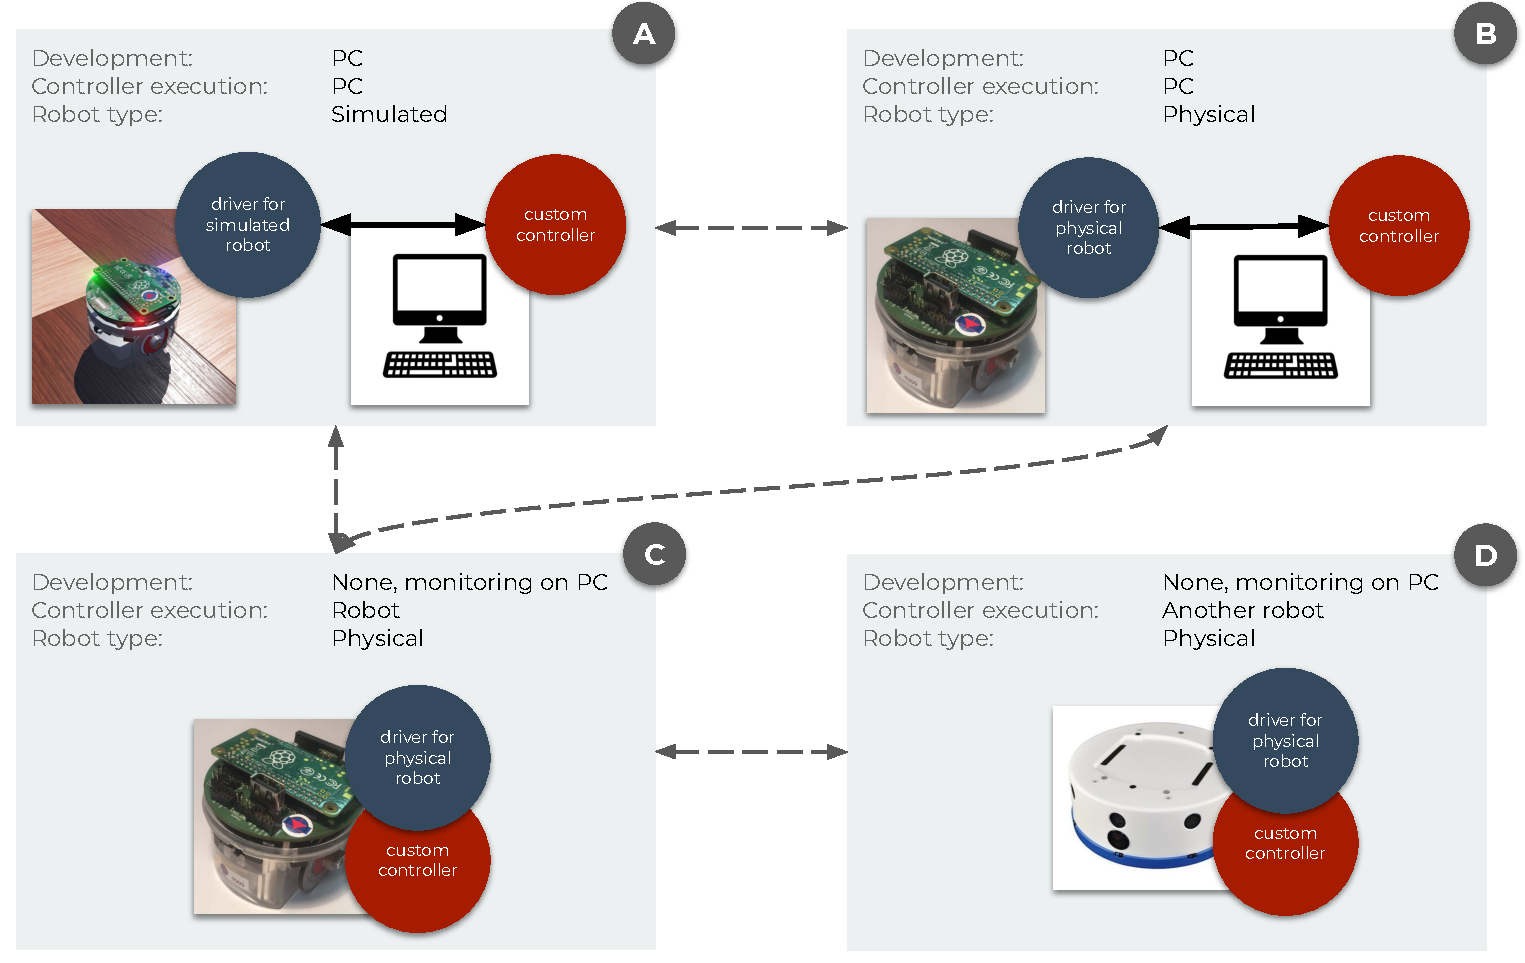
\includegraphics[width=\textwidth]{introduction/figures/desired_workflow.pdf}
    \caption{A development workflow (in robotics) that has to be achieved with the proposed solution. The circle represents a piece of software that the user wants to develop to control the robot, and it is the same in each scenario. The dashed arrows are transitions in the development workflow, while solid the solid arrows represent a network protocol.}
    \label{fig:introduction:desired_workflow}
\end{figure}

In Fig. \ref{fig:introduction:desired_workflow} the user develops a robot controller called \texttt{custom controller}. From the user's perspective, the controller supposed to be the same in each scenario. First, the user should start by developing the controller on PC and testing it in the simulation. After the user is satisfied with the simulation's behavior, the controller can still be executed on the PC, but now it can control the physical robot. If the robot's behavior is not desired, the user can improve the simulation model and test it again in the simulation, reducing the simulation and the real-world gap. Once everything works as expected, the user should move the controller to the robot. Here, it is possible, e.g., to hit the computational limit of the on-board computer, and the controller should be edited and tested again in the simulation, moving back to the on-board computer once it is ready. Finally, the controller can be shared with the other researchers to evaluate the other robots' control software or further improve it.

The project has to be done in three phases. First, a specific \ac{ros2} nodes for an e-puck2 simulated and physical robot have to be developed. Second, examples that utilize the nodes have to be created. The purpose of this phase is to evaluate the nodes and to give the users usage examples. Finally, in the third phase, the specific \ac{ros2} node for e-puck2 simulated robot has to be generalized to support other robots, focusing on Khepera IV robot. The final software has to be peer-reviewed, united tested, code quality tested, automated with \ac{ci}\footnote{The \ac{ci} automation has to be done with Industrial CI. This \ac{ci} is created by ROS-industrial, an organization committed to close a gap between research and industry by bringing industry standards to \ac{ros2}}, user friendly, and well documented with comprehensive tutorials.

\section{Document Structure}
% Inspired by:
% - https://essay.utwente.nl/59475/1/scriptie_R_van_Domburg.pdf
% - http://www.jedlitschkas.de/downloads/jedlitschka_etAl_reporting.pdf

The structure of the thesis roughly follows the phases described in the previous section. It should allow readers to skip information, but also to reduce the chance of missing important details. Therefore, the project is presented as follows:

\begin{itemize}
    \item \textbf{Chapter \ref{chap:background}: \nameref{chap:background}} gives the theoretical background on common concepts, and software and hardware technologies, utilized in the project. Also, it clarifies relations with relevant projects.
    
    \item \textbf{Chapter \ref{chap:simulation}: \nameref{chap:simulation}} explains a process used to create a \ac{ros2} node that exposes access to simulated e-puck2 robot's sensors and actuators through \ac{ros2} interface.
    
    \item \textbf{Chapter \ref{chap:physical}: \nameref{chap:physical}} has a goal to explain implementation of the same \ac{ros2} interface for e-puck2 physical robot.
    
    \item \textbf{Chapter \ref{chap:demos}: \nameref{chap:demos}} shows tools, existing packages and custom created controllers that utilize the e-puck2 \ac{ros2} interface.
    
    \item \textbf{Chapter \ref{chap:generalization}: \nameref{chap:generalization}} gives implementation overview on generalized \ac{ros2} driver for simulated robot. It aims to extend e-puck2 driver to support Khepera IV, TurtleBot 3 Burger and potentially the other robots as well.
    
    \item \textbf{Chapter \ref{chap:results}: \nameref{chap:results}} quantifies difference between the \ac{ros2} driver for the simulated and the physical robot, difference between e-puck2 and Khepera IV \ac{ros2} interfaces and it shows simplification resulted by generalization described in the previous chapter.
    
    \item \textbf{Chapter \ref{chap:conclusion}: \nameref{chap:conclusion}} presents the project summary, limitations, impact and potential improvements.
\end{itemize}}{}
\iftoggle{FULL_REPORT}{\chapter{Background and Related Work}
\label{chap:background}
\shorttitle{\nameref{chap:background}}

This chapter has two purposes.
First, to give a reader a theoretical background about concepts and technologies needed for understanding the project.
Second, it shows the related work - how this project is different and what improvements it brings in comparison to the existing solutions.

\section{\ac{ros}}

The initial founders of \ac{ros} define it as an open-source operating system, that, instead of process management and scheduling, provides a communication layer on top of the host operating systems of a heterogeneous compute cluster \cite{quigley_ros_nodate}.

\begin{figure}[H]
    \centering
    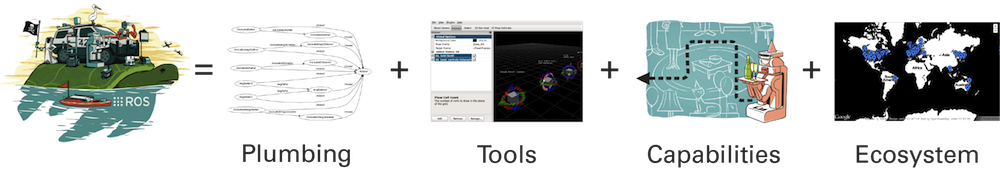
\includegraphics[width=\textwidth]{background/figures/ros_equation.png}
    \caption{\ac{ros} described through a picture, available at the official \ac{ros} website}
    \label{fig:background:ros_equation}
\end{figure}

One also can say that \ac{ros} is a collection of tools, libraries, and conventions that simplify developing a complex robot behavior.
In one interview, Roger Barga, leader of an Amazon's Web Service (AWS RoboMaker), emphasized the importance of \ac{ros} in robotics by saying \textit{``We think that ROS is becoming the Linux for the robots of the future''}\footnote{Roger Barga is an interview by Ricardo Tellez (from The Construct) in ROS Developers podcast -    \url{https://www.theconstructsim.com/aws-robomaker-with-roger-barga/}.}.
Defining \ac{ros} in one sentence is hard, but in further text, two crucial concepts of \ac{ros} will be covered.

The first is the concept of a node.
A task of the node is to perform a computation.
The nodes utilize a publisher-subscriber communication model to exchange messages with each other. 
In that way, the nodes are combined into a graph that can perform more complex tasks.
There are a few important characteristics of each node:
\begin{itemize}
    \item The node can be implemented in various programming languages, without affecting the other nodes.
    Being programming language agnostic allows developers to optimize the nodes for different behaviors.
    For example, if the node has to be efficient or interact closely with the hardware C programming language may be more suitable.
    Otherwise, if fast prototyping is important,  Python may be a better fit.
    As a result, community nodes are implemented in a programming language that fits best the node's purpose.
    \item The nodes can be run on different computers.
    Each \ac{ros} node includes a mechanism to communicate locally or over the network with the other nodes.
    A complex robotics system often includes multiple powerful computers and dozens of \acp{mcu} or \acp{fpga} specialized for various tasks, and therefore, this ability of \ac{ros} nodes is significant.
    In this project, for example:
    \begin{itemize}
        \item \ac{mcu} is used to execute real-time tasks, like motor control,
        \item on-board computer is used heavy tasks, like perception,
        \item while workstation (\acs{pc}) is used for data visualization, monitoring and debugging.
    \end{itemize}
    \item The nodes can run on virtually any \ac{os}.
    Since \ac{ros2}, Linux, Mac, and Windows are officially supported.
    A stripped version of \ac{ros2}, micro-ROS, runs even on NuttX, FreeRTOS, and Zephyr, and the community has been porting to other \acp{os} as well.
    \item Since \ac{ros2}, the nodes are fully distributed. 
    It means that there is no single message broker to orchestrate the communication.
    Being distributed significantly increases robustness as there is no single point of failure if a node crashes the rest of the system will continue to function.
\end{itemize}

In Fig. \ref{fig:background:ros_nodes} a graph of \ac{ros} nodes is given representing the node concepts given before.

\begin{figure}[H]
    \centering
    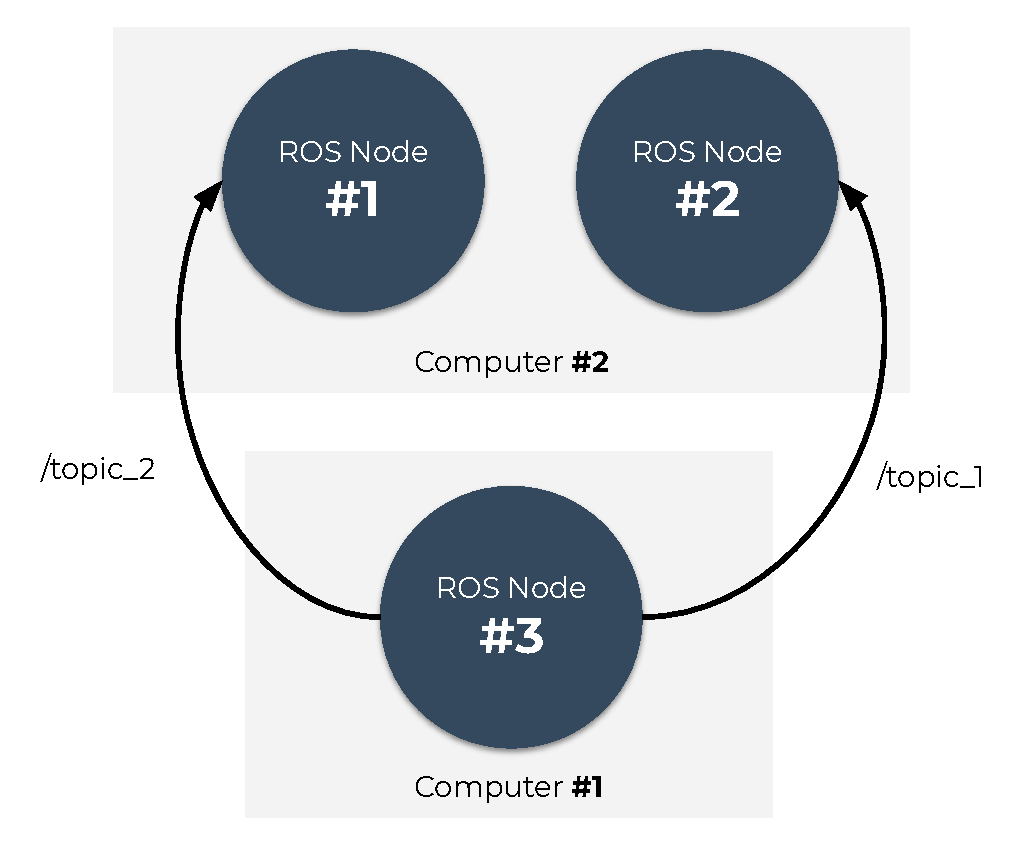
\includegraphics[width=0.8\textwidth]{background/figures/ros_nodes.pdf}
    \caption{General example of three nodes exchange messages through two topics}
    \label{fig:background:ros_nodes}
\end{figure}


The second important concept in \ac{ros} is the means of communication between the nodes.
Mostly, communication between nodes is done through topics, but there other types of communication:
\begin{itemize}
    \item Topics use publisher-subscriber communication model \cite{chen_beaconvey_2018}.
    It means that a node's message will be received by all nodes that are subscribed to the corresponding topic. 
    \ac{qos} was important to \ac{ros} team and therefore, the following \ac{qos} can be defined:
    \begin{itemize}
        \item history, keep last (keep only the last N messages) or keep all,
        \item reliability, best effort (may lose messages if the network is not stable) or reliable (guarantees message delivery) and
        \item durability, transient local (nodes that got subscribed to a topic will receive the last message even though the message is published long time before) or volatile (messages will not be preserved for late-joiners).
    \end{itemize}
    \item Services are used to get a response from the other nodes.
    The concept is very similar to functions with return values.
    A client node sends a service request with data to a node that provides service, and after the result is ready the client node gets the response.
    A typical request can be, \textit{``Is the motor turned on?''} or \textit{``Retrieve the full map now''}.
    \item Parameters allow nodes to be configured by the user or other nodes, on startup or during run-time.
    The underlying implementation is based on the previously explained services.
    I means the nodes can be configured over the network.
    \item Actions are available since \ac{ros2}, and they are similar to the services.
    A difference is that the actions are optimized for requests that generally take longer to execute and need continuous feedback. A typical action can be, \textit{``Move the robot to the new position and while doing it, keep sending me a position''}.
\end{itemize}

The nodes and means of communication between the nodes, are two core concepts of \ac{ros} around which all \ac{ros} tools are built.
Depending on the area of robotics, new concepts may also emerge, but those two are the foundation of the \ac{ros}.

%TODO: \subsection{\ac{ros} Packages}
%TODO: \subsubsection{tf2}
%TODO: \subsection{\ac{ros} Middleware}
%TODO: ROS1 vs ROS2 table


\subsection{\ac{ros} Messages}
One of the sub-objectives of this master project is to provide \ac{ros2} interface that is as compatible as possible with the existing packages.
That will allow users to simply integrate existing \ac{ros2} packages and significantly increase their productivity.
To achieve the objective, \ac{ros2} defines a vast list of existing message, service, and action types.
In the scope of the project, only message types will be further described.

Except for the standard types, available in most programming languages, such as bool, integer, float and string, some messages are more specific to the robotics such as odometry (for describing odometry data), twist (for defining angular and linear velocity), and range (for data from distance sensors).
These messages are exchanged through the previously described topics.
Therefore, integrating a community \ac{ros2} package is a matter of launching (and sometimes configuring it), the package should automatically start publishing and subscribing to the messages as common message types are used.

There are a few groups of message types, some of which are:
\begin{itemize}
    \item \texttt{std\_msgs} is a wrapper around primitive types such as \texttt{Bool}, \texttt{Int32}, \texttt{Float64}, \texttt{String} and \texttt{Float64MultiArray}.
    These message types are usually used to compose more complex message types and in general should be avoidable if there is more suitable type from the other groups.
    \item \texttt{geometry\_msgs} contains geometry primitives.
    For example \texttt{Twist} is used to describe linear and angular velocity (usually used to control robot's velocity), rotations are described with \texttt{Quaternion} message types, robot's pose \texttt{Pose} (e.g. the navigation stack uses this message type describe the robot's goal position and orientation) and \texttt{Transform} to describe relative orientation and translation of two frames.
    \item \texttt{nav\_msgs} group contains message types used to interact with the navigation stack and the related packages.
    It defines message types such as \texttt{OccupancyGrid} that represent a map and \texttt{Odometry} that contains odometry data. 
    \item \texttt{sensor\_msgs} contains message types that are commonly used to describe data from sensor such as distance sensors (\texttt{Range}), \acsp{lidar} (\texttt{LaserScan}), cameras (\texttt{CameraInfo} and \texttt{Image}), light sensors (\texttt{Illuminance}) and similar. 
\end{itemize}

There are many more message group types, but those are the most relevant ones for this project.

\subsection{\ac{ros} Distributions}

\ac{ros} distributions is another vital aspect of the project.
The newest \ac{ros} distribution, as of the time of witting this, is deliberately chosen.
The choice is will be described later, but first, \ac{ros} versioning has to be described.

\ac{ros} team releases a new \ac{ros} distribution every six months, following Ubuntu's release cycle.
Every two years a new \ac{ros} \ac{lts} is released,
a few weeks after Ubuntu's \ac{lts} release, as \ac{ros} relies on the latest Ubuntu \ac{lts}.

In December 2017, \ac{ros2} is introduced, and since then \ac{ros} team has been publishing \ac{ros} and \ac{ros} releases every six months.
\ac{ros2} should fully replace the \ac{ros1} once \ac{ros2} mature\footnote{Dirk Thomas, principle software engineer working on \ac{ros} core, wrote about \ac{ros} future at \ac{ros} Discourse -  \url{https://discourse.ros.org/t/planning-future-ros-1-distribution-s/6538}. He stated \ac{ros1} will be most probably supported until 2025 and then it should be completely replaced by \ac{ros2}}.

\begin{figure}[H]
    \centering
    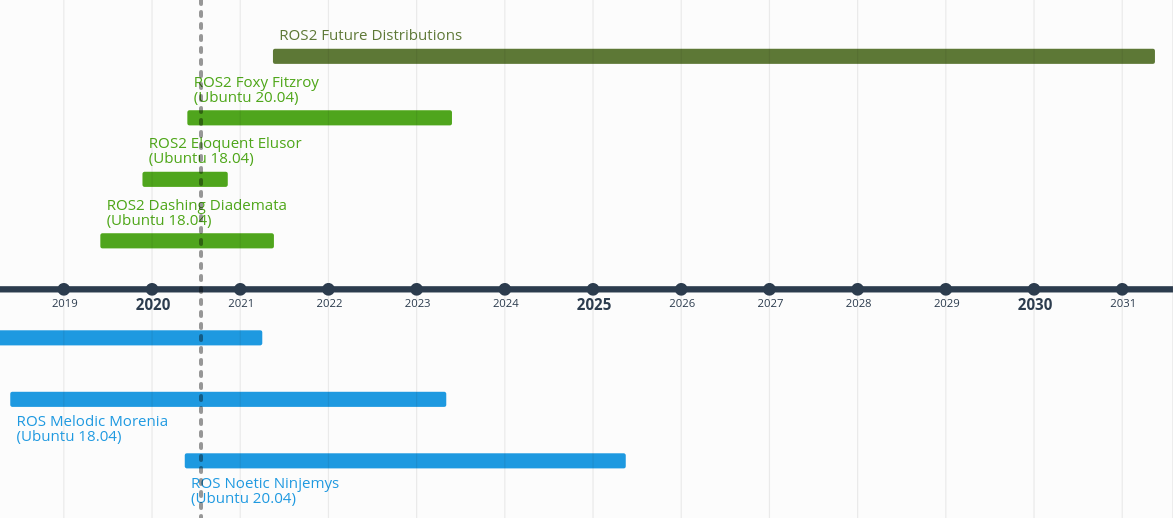
\includegraphics[width=\textwidth]{background/figures/ros_distributions.png}
    \caption{Timeline of \ac{ros1} and \ac{ros2} distributions}
    \label{fig:background:ros_distributions}
\end{figure}

In Fig. \ref{fig:background:ros_distributions} a few latest \ac{ros} distributions are shown.
Note that they all rely on Ubuntu \ac{lts} distributions and that \ac{ros2} Foxy Fitzroy is the first \ac{ros2} distribution with three years of support.

In this project, the importance of \ac{ros2} is recognized, and therefore it is chosen instead of \ac{ros1}.
Also, the master project had started before \ac{ros2} Foxy Fitzroy was released, and therefore the initial code is written for \ac{ros2} Eloquent Elusor with a plan to adopt \ac{ros2} Foxy Fitzroy.
Finally, the master project is compatible with \ac{ros2} Eloquent Elusor and \ac{ros2} Foxy Fitzroy.

\section{Robotics Platforms}
The project's main objective is to introduce \ac{ros2} support for the e-puck2 physical and simulated robot, and other simulated robots while focusing on Khepera IV.
Therefore, those two robots is will be described in more detail.

\subsection{E-puck2}
E-puck2 is the second generation of the e-puck robot\cite{mondada_e-puck_nodate}.
E-pucks are small differential wheeled robots (e-puck and e-puck2 have the same footprint) with a radius of 35mm.
As a miniature robot, it is the perfect candidate for education and multi-robot research.
It is originally designed for micro-engineering education by Michael Bonani and Francesco Mondada at \ac{epfl}.
The robot is open hardware, and the software is open-source.

\begin{figure}[H]
    \centering
    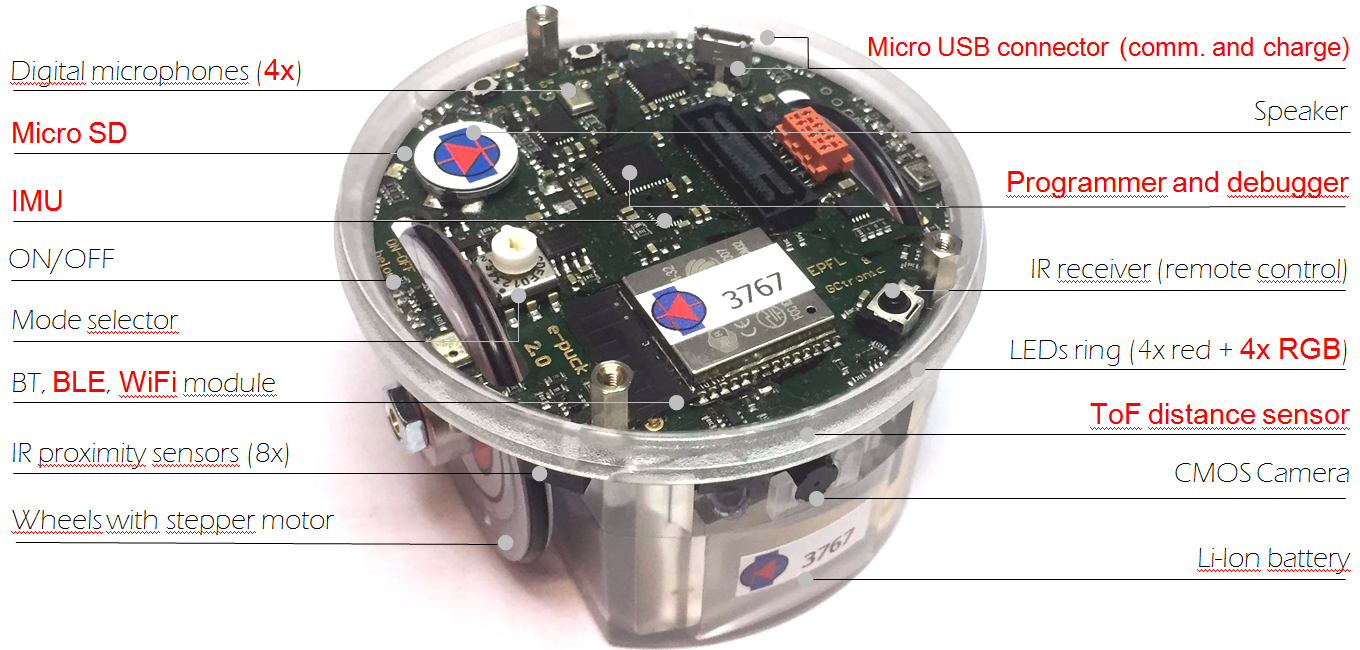
\includegraphics[width=\textwidth]{background/figures/e-puck2-features.png}
    \caption{E-puck2 robot with list of main components (taken from the official website)}
    \label{fig:background:e-puck2}
\end{figure}

The robot is shown in Fig. \ref{fig:background:e-puck2} and its main specifications are given in Table. \ref{tab:background:specifications}.

\begin{table}[H]
    \begin{adjustwidth}{-1.5in}{-1.5in}
    \centering
    \begin{tabular}{|l|l|}
        \hline
        Size, weight & 70mm diameter, 130g \\
        \hline
        \ac{mcu} & 32-bit STM32F407 @ 168 MHz (210 \acs{mips}), \acs{dsp} and \acs{fpu}, \acs{dma} \\
        \hline
        Motors & 2 stepper motors, 50:1 reduction gear and 20 steps per revolution \\
        \hline
        Max velocity & 0.154m/s \\
        \hline
        Distance sensor & 8 infra-red sensors (up to 0.06m) and one \acs{tof} (up to 2m) \\
        \hline
        Camera & 640x480 at 15\acs{fps} \\
        \hline
        \acs{imu} & 3D accelerometer, 3D gyro, 3D magnetometer \\
        \hline
        \acsp{led} & 4 red \acsp{led} and 4 \acs{rgb} \acsp{led} \\
        \hline
    \end{tabular}
    \end{adjustwidth}
    \caption{Relevant specifications of e-puck2 robot}
    \label{tab:background:specifications}
\end{table}

\subsubsection{Pi-puck}

E-puck2 robot allows extensions to be added providing different features such as additional autonomy, ground sensors or additional processing power.
The pi-puck extension, for example, consists of a Raspberry Pi Zero W and adapter \ac{pcb}, and interacts directly with on-board \ac{mcu} and sensors \cite{millard_pi-puck_2017}.
Since Raspberry Pi Zero W is Linux base board it can run \ac{ros} with full \ac{dds} implementation.

\begin{figure}[H]
    \centering
    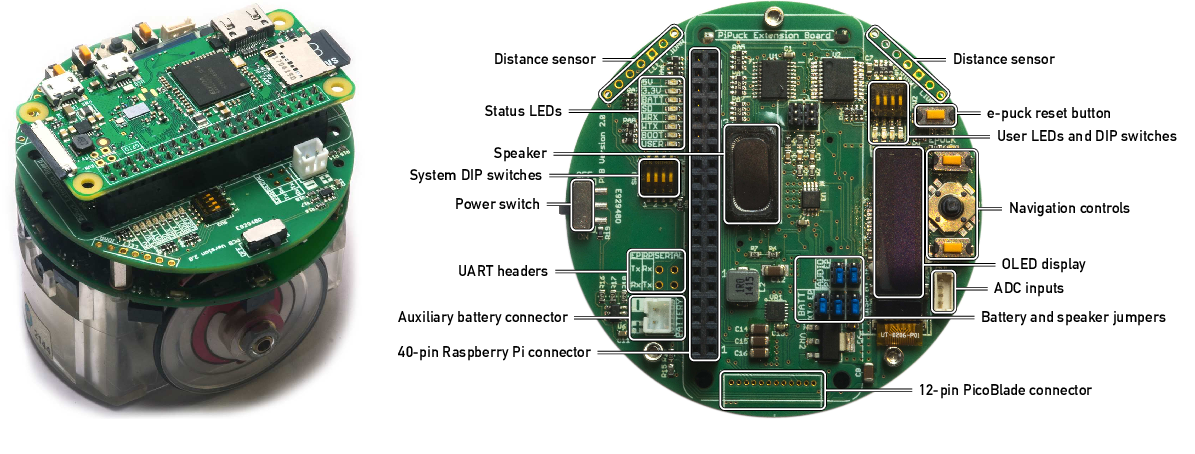
\includegraphics[width=\textwidth]{background/figures/pi-puck.png}
    \caption{Pi-puck extension consist of two parts, \ac{pcb} and Raspberry Pi Zero W \cite{millard_pi-puck_2017}}
    \label{fig:background:pi-puck}
\end{figure}

In the project, Raspberry Pi Zero W allows us to run \ac{ros2} nodes on the robot and execute complex operations such as \acs{jpeg} image compression that otherwise would not be possible.

\subsection{Khepera IV}

Khepera IV is a similar robot to e-puck2, but is more prominent in size (with a radius of 70mm), and has more powerful sensors and computational units \cite{reis_khepera_2016}.
The robot is designed by K-Team\footnote{Official website of K-Team is available at \url{https://www.k-team.com/}.} to fit any indoor lab application.

\begin{figure}[H]
    \centering
    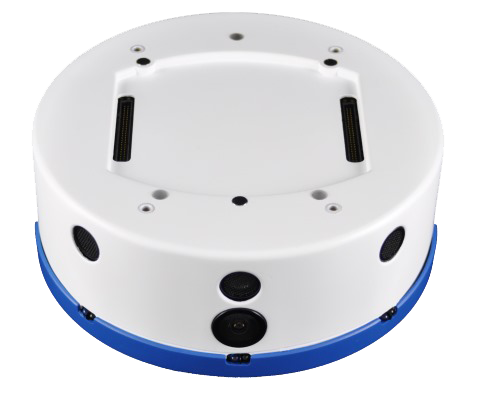
\includegraphics[width=0.6\textwidth]{background/figures/khepera_iv.png}
    \caption{Khepera IV robot \cite{reis_khepera_2016}}
    \label{fig:background:khepera_iv}
\end{figure}

The robot is shown in Fig. \ref{fig:background:khepera_iv} and its main specifications are given in Table. \ref{tab:background:khepera_iv}.

\begin{table}[H]
    \centering
    \begin{tabular}{|l|l|}
        \hline
        Size, weight & 140mm diameter, 540g \\
        \hline
        Processor & 800MHz ARM Cortex-A8 Processor and \acs{mcu} \\
        \hline
        Motors & 2 DC brushed motors with incremental encoders \\
        \hline
        Max velocity & 0.8m/s \\
        \hline
        Distance sensor & 8 infra-red (up to 0.25m) and 5 ultrasonic (up to 2m) \\
        \hline
        Camera & 752x480 at 30\acs{fps} \\
        \hline
        \acs{imu} & 3D accelerometer, 3D gyro \\
        \hline
        \acsp{led} & 3 \acs{rgb} \acsp{led} \\
        \hline
    \end{tabular}
    \caption{Relevant specifications of Khepera IV robot}
    \label{tab:background:khepera_iv}
\end{table}

\section{Webots}
Webots is an open-source robot simulator developed by Cyberbotics\footnote{Official website of Cyberbotics is available at \url{https://cyberbotics.com/}.}, initially designed at \ac{epfl}.
The simulator provides a development environment to model, program and simulate robots \cite{michel_cyberbotics_2004, michel_webots_1998, michel_cyberbotics_2014}.

\begin{figure}[H]
    \centering
    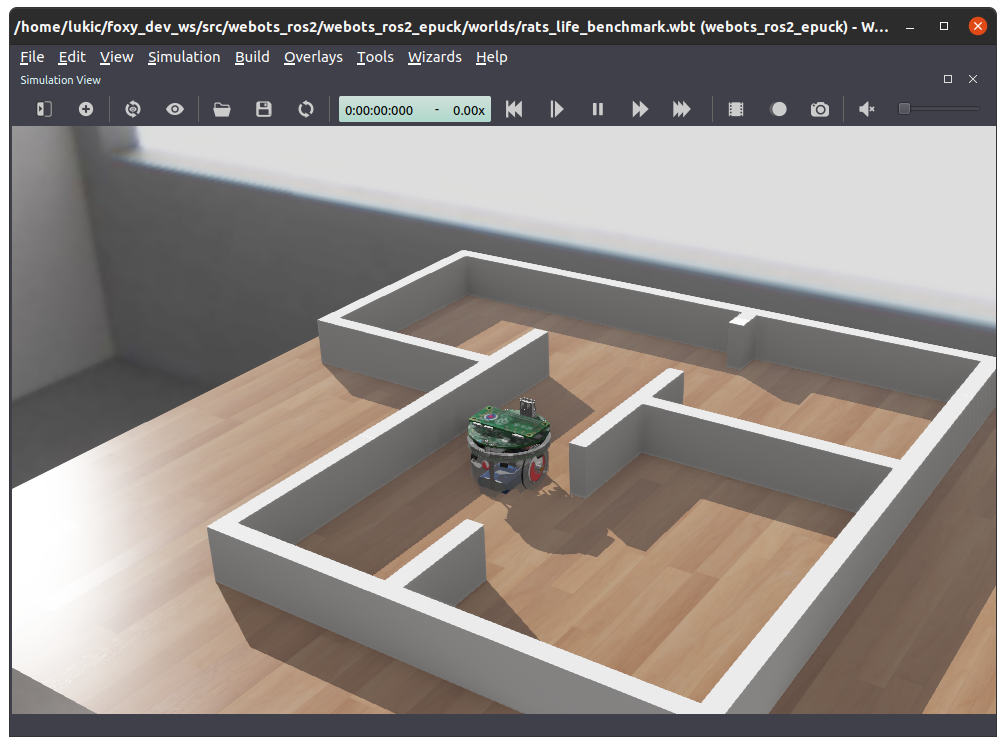
\includegraphics[width=\textwidth]{background/figures/webots.png}
    \caption{Webots robot simulator: e-puck2 robot on a table}
    \label{fig:background:webots}
\end{figure}

The main Webots features are:
\begin{itemize}
    \item Robot/world editor: The models are stored in VRML97 format, allowing users to either change the document directly or through the Webots user interface. 
    The Webots world editor allows the users to see changes in the world immediately.
    It is possible to include pre-built models, and the users can choose among a huge library of models.
    \item Realistic simulation: The simulations produced in Webots are realistic compared to the similar products. 
    The physics simulation is based on a modified version of \ac{ode}.
    The models shipped with the Webots are visually very detailed, although still optimized for high performance.
    \item Programming interface: \ac{api} for programming robots is officially available in the most popular programming languages, C, C++, Python, MATLAB and Java, while community-contributed packages further extend this list\footnote{An example of \ac{api} in Haskell programming language, created by the community, is available at \url{https://github.com/cyberbotics/HsWebots}.}.
    The \ac{api} allows simple access to the sensors and actuators available in the robots.
    \item Deterministic simulations: Webots guarantees a simulation to output the same behavior every time it runs (user can also choose non-deterministic simulation).
    Although a non-deterministic simulation is preferable before transferring to a real robot, deterministic simulation is beneficial when doing initial algorithm tests.
    Also, this feature can be exploited to simplify automated testing in \ac{ci}.
\end{itemize}

Those are the main points that justify the usage of Webots over similar products.

\section{Related Work}
Existing \ac{ros} support for the e-puck2 physical robot and Webots will be analyzed.
Drawbacks in current implementations of \ac{ros} support are the motivation for this project; therefore, they will be explained in this section.

\subsection{\ac{ros} Support for E-puck2}
GCtronic, a company behind e-puck robots, has two types of \ac{ros} drivers available.
The first is made for e-puck robots without pi-puck extension\footnote{\ac{ros} driver that doesn't run on pi-puck extension is available at \url{https://github.com/gctronic/epuck_driver_cpp/tree/e-puck2}.}.
In that case, \ac{ros} driver runs on a workstation while communicating with the e-puck over Bluetooth. The second \ac{ros} driver implementation runs on pi-puck extension\footnote{\ac{ros} driver that uses pi-puck extension is available at \url{https://github.com/gctronic/epuck_driver_cpp/tree/pi-puck}.} and it is similar to the \ac{ros} driver we aim to develop. The main drawbacks are that it is not available for \ac{ros2}, it is not unit tested nor code quality tested, it does not include a camera driver, and there is no comprehensive documentation.

\begin{table}[H]
    \begin{adjustwidth}{-1.5in}{-1.5in}
    \centering
    \begin{tabular}{|l|c|c|c|}
         \hline
         & \textbf{GCtronic's \#1} & \textbf{GCtronic's \#2} & \textbf{Proposed solution} \\
         \hline
         \rowcolor{lightgray} \textbf{\ac{ros2} support} & No & No & Yes \\
         \hline
         \rowcolor{lightgray} \textbf{Communication} & Bluetooth & \acs{udpros}/\acs{tcpros} & \ac{dds} \\
         \hline
         \rowcolor{lightgray} \textbf{Camera} & 160x120@4 & No & 640x480@10 \\
         \hline
         \textbf{Battery autonomy} & Long & Short & Short \\
         \hline
         \rowcolor{lightgray} \textbf{Unit tests} & No & No & Yes, with \ac{ci} \\
         \hline
         \rowcolor{lightgray} \textbf{Code quality tests} & No & No & Yes, with \ac{ci} \\
         \hline
         \rowcolor{lightgray} \textbf{Cross-compilation} & No & No & Yes, tools are given  \\
         \hline
         \rowcolor{lightgray} \textbf{Independent from \acs{pc}} & No & Yes & Yes  \\
         \hline
    \end{tabular}
    \end{adjustwidth}
    \caption[Comparison of the proposed \ac{ros} drive with the existing implementations]{Comparison of the proposed \ac{ros2} driver with the existing implementations (aspects in which the proposed solution is better are highlighted).}
    \label{tab:background:epuck_ros}
\end{table}

As showed in Table \ref{tab:background:epuck_ros} the proposed solution offers better implementation in many aspects.
The proposed solution's main drawback is the battery autonomy as the pi-puck extension requires a significant amount of power (around 0.7 watts, it can vary depending on usage).


\subsection{\ac{ros} Support in Webots}
A major part of the master project is the improvement of \ac{ros2} support for Webots.
Webots supports both, \ac{ros1} and \ac{ros2}, but with certain limitations.

Webots \ac{ros1} implementation automatically exposes all Webots \ac{api} functions as \ac{ros} topics and services.
Automatically exposing \ac{ros} \ac{api} sounds as a reasonable solution, but it is uncanny for the \ac{ros} ecosystem, and therefore, much effort is required from users to adapt the exposed \ac{api} to fit other \ac{ros} packages.
For example, if one wants to publish odometry data, the one needs to create a \ac{ros} node that subscribes topics published by encoders and then publishes the corresponding odometry and transform messages. This work is time consuming, complex, and consumes unnecessary processing power by republishing all the messages.

Therefore, Cyberbotics has taken another approach in \ac{ros2} support.
Instead of creating \ac{ros2} topics and services as done for \ac{ros1} it provides facilities to users to design and implement their own \ac{ros2} interface using Webots \ac{api} functions.
Creating a specific \ac{ros2} driver simplifies usage, but it is still time-consuming as the \ac{ros2} driver has to be created for each robot.

This project extends Webots' support for \ac{ros2} by adding modules that can automatically create \ac{ros2} interface, compatible with other \ac{ros2} packages, based on a robot description.
For the previously mentioned example, in which odometry has to be published, the proposed improvement will allow automatic publishing of odometry and transform messages, including support for \ac{ros2} parameters and velocity control of the robots.

This improvement should allow users to integrate Webots simulations faster in their \ac{ros2} applications, and it should effectively lead to a greater adoption of robot simulations among the \ac{ros2} community that uses Webots.
}{}
\iftoggle{FULL_REPORT}{\chapter{E-puck2 Simulation and \acs{ros2} Interface}
\label{chap:simulation}
\shorttitle{\nameref{chap:simulation}}

As previously explained, one of the project's objectives is to create a \ac{ros2} interface for simulated e-puck2 robots.
Even though creating \ac{ros2} interface for Webots robots is automated later in the project, specific \ac{ros2} driver for the e-puck2 in Webots is created first.
For us as developers, creating the specific \ac{ros2} driver was necessary to understand better building blocks that can be generalized.
To readers, this chapter will help better understand improvements brought by generalization (see Chapter \ref{chap:generalization}).
It will also show that some devices cannot be generalized, e.g., distance sensors cannot feed the \texttt{LaserScan} topic.

\section{Introduction}

Before going to implementation details, it is important to understand the concept of a controller in Webots and how it fits in \ac{ros2} driver for Webots simulated robots.
The Webots controller controls actuators and reads data from sensors available in a robot.
The controller is a "brain" of the robot; it makes the robot move and senses the environment.
It consists of two parts, the Webots \ac{api}, which communicates with the simulation and user-defined code that uses that Webots \ac{api} to control the robot.
The Webots \ac{api} communicates with the Webots simulation through pipes, a type of inter-process communication \cite{kashyian_portable_2008}.
Therefore, there are two processes that run independently, Webots controller and Webots simulation (see Fig. \ref{fig:simulation:webots_user_code_and_api}).

\begin{figure}[H]
    \centering
    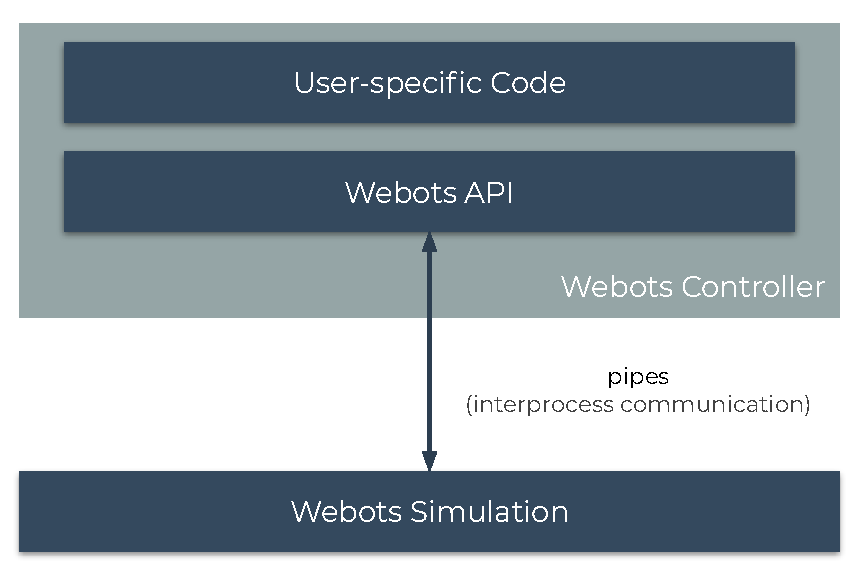
\includegraphics[width=0.8\textwidth]{simulation/figures/webots_user_code_and_api.pdf}
    \caption{User specific code, \ac{api} and simulation within Webots}
    \label{fig:simulation:webots_user_code_and_api}
\end{figure}

In this chapter, a logic that performs translation from Webots \ac{api} to \ac{ros2} \ac{api} will be implemented as a Webots controller (block \textit{User-specific Code} in Fig. \ref{fig:simulation:webots_user_code_and_api}).
Therefore, a block \textit{Webots Controller} from the figure will be referenced as \ac{ros2} driver in the further text.

\section{Webots within \ac{ros2}}
As \ac{ros2} driver is defined, we should clarify how the \ac{ros2} driver and Webots simulation can be launched within a \ac{ros2} application. 
The straightforward way to launch the \ac{ros2} driver and Webots simulation is the following:
\begin{itemize}
    \item put \ac{ros2} libraries to the environment variable \texttt{PATH},
    \item start the Webots simulation,
    \item execute the \ac{ros2} driver and
    \item start the rest of the \ac{ros2} application (\ac{ros2} nodes).
\end{itemize}

However, to better integrate Webots into \ac{ros2}, launch files\footnote{Launch files in scope of \ac{ros2} are poorly documented. Good documentation to understand the core concepts (although not completely accurate) can be found in \ac{ros2} design specification at \url{https://design.ros2.org/articles/roslaunch.html}. A superficial explanation, hiding core concepts, on the usage of the launch files, is given in \ac{ros2} tutorials at \url{https://index.ros.org/doc/ros2/Tutorials/Launch-system/}.} are used. The launch files in \ac{ros2} allow user to execute multiple processes (often \ac{ros2} nodes) at once. The launch files are described with Python scripts, and there are three important concepts:
\begin{itemize}
    \item Actions: They represent an intention to do something, like start a process (usually \ac{ros2} nodes), set a parameter, or push a namespace. 
    \item Substitutions: Define a transformable expression. 
    It means that the expression contains a placeholder that can be replaced.
    For example, the substitution can be a path to a file in which filename is again a substitution: \\ \texttt{PathJoinSubstitution([package\_path, LaunchConfiguration('world')])}
    \item Events: Actions can produce subscribable events.
    For example, when a process is closed, it will emit an event on which we can close the whole \ac{ros2} application.
\end{itemize}

Using those three concepts a minimal launch file containing Webots and \ac{ros2} driver is created (see Fig. \ref{fig:simulation:webots_launch}).

\begin{figure}[H]
    \centering
    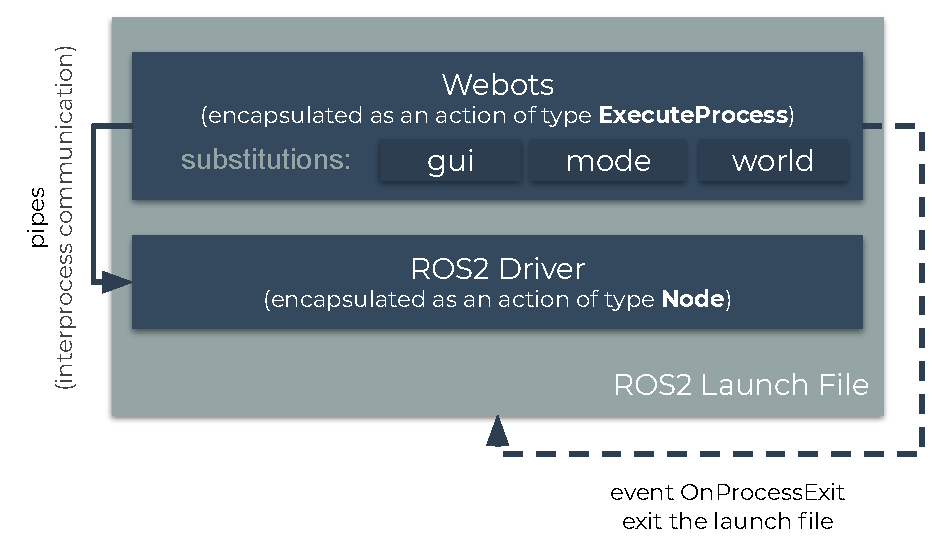
\includegraphics[width=\textwidth]{simulation/figures/webots_launch.pdf}
    \caption{Webots and \ac{ros2} driver within the launch file}
    \label{fig:simulation:webots_launch}
\end{figure}

It will start Webots with three substitutions, \texttt{gui}, \texttt{mode} and \texttt{world} which are used to configure Webots.
These substitutions are taken from arguments (as \texttt{LaunchConfiguration}).
Also it defines an action which will kill the launch file if the user exit the simulation.

This whole implementation is later completely hidden from the user (introduced in Chapter \ref{chap:generalization}).

% TODO: Explain clock synchronization

\section{Covered Sensors and Actuators}

In this section, the implementation of \ac{ros2} driver for the simulated e-puck2 robot is explained.
Please note that only the first section (Section \ref{sec:simulation:odometry_velocity}) will provide the comprehensive explanation of the respective topic.
The other sections will only briefly cover the implementation details as the \ac{ros2} support does not differ significantly from sensor to sensor.
It is essential to choose a suitable message type and thoroughly format data accordingly.

\subsection{Differential Drive}
\label{sec:simulation:odometry_velocity}

Using data from sensors such as wheel encoders, camera, or \ac{imu}, or fusing them, one can estimate the change in robot's position overtime \cite{shen_localization_2011, nister_visual_2004}.
With the dead reckoning method, the change in position can be accumulated, and in that way, the robot's position in the local frame (frame relative to the robot's start position) can be estimated \cite{ben-ari_elements_2018, astolfi_exponential_1999}.
In \ac{ros2}, each sensor used for odometry should publish messages of type \texttt{nav\_msgs/Odometry}, and messages from different sensors later can be fused to increase accuracy. 

In the scope of this project, only wheel encoders are used for odometry.
Furthermore, the e-puck2 does not have encoders but step motors.
However, since we can control steps precisely, that data can be used for odometry calculation.

\begin{figure}[H]
    \centering
    \begin{subfigure}[b]{0.9\textwidth}
        \dirtree{%
            .1 nav\_msgs/Odometry.
            .2 (std\_msgs/Header) header.
            .2 (string) child\_frame\_id.
            .2 (geometry\_msgs/PoseWithCovariance) pose.
            .3 (geometry\_msgs/Pose) pose.
            .4 (geometry\_msgs/Point) position.
            .4 (geometry\_msgs/Quaternion) orientation.
            .3 (float64[36]) covariance.
            .2 (geometry\_msgs/TwistWithCovariance) twist.
            .3 (geometry\_msgs/Twist) twist.
            .4 (geometry\_msgs/Vector3) linear.
            .4 (geometry\_msgs/Vector3) angular.
            .3 (float64[36]) covariance.
        }
    \end{subfigure}
    \caption{\texttt{nav\_msgs/Odometry} message type definition in \ac{ros2}}
    \label{fig:simulation:odometry}
\end{figure}

In Fig. \ref{fig:simulation:odometry}, odometry format proposed by \ac{ros2} and used by the community packages is given. It requires \texttt{geometry\_msgs/Pose} (position and orientation) of the robot to be specified, as well as \texttt{geometry\_msgs/Twist} (linear and angular velocity).

First we express velocity of left ($v_left$) and right ($v_right$) wheel by multiplying wheel radius ($R$) with angular velocity:
\begin{equation}
\begin{aligned}
    v_{left} = R \frac{\gamma_{left}(n) - \gamma_{left}(n-1)}{\Delta t} \\
    v_{right} = R \frac{\gamma_{right}(n) - \gamma_{right}(n-1)}{\Delta t}
\end{aligned}
\end{equation}
in which $ \gamma_{left}(n) $ and $ \gamma_{right}(n) $ are angular positions of left and right wheel respectively at the sample $ n $.

For differential drive robots we can simply express linear ($v$) and angular ($\omega$) velocity as:
\begin{equation}
\begin{aligned}
    v = \frac{v_{left} + v_{right}}{2}  \\
    \omega = \frac{v_{right} - v_{left}}{L}
\end{aligned}
\end{equation}
where $ L $ is axle length (distance between the left and the right wheel). The velocity of the robot in odometry frame is given by:
\begin{equation}
\begin{bmatrix}
\dot{x} \\
\dot{y} \\
\dot{\theta}
\end{bmatrix} = \begin{bmatrix}
v \cos(\theta) \\
v \sin(\theta) \\
\omega
\end{bmatrix}
\end{equation}

Knowing the angular and linear velocity, we can integrate it to obtain a position.

\begin{figure}[H]
    \centering
    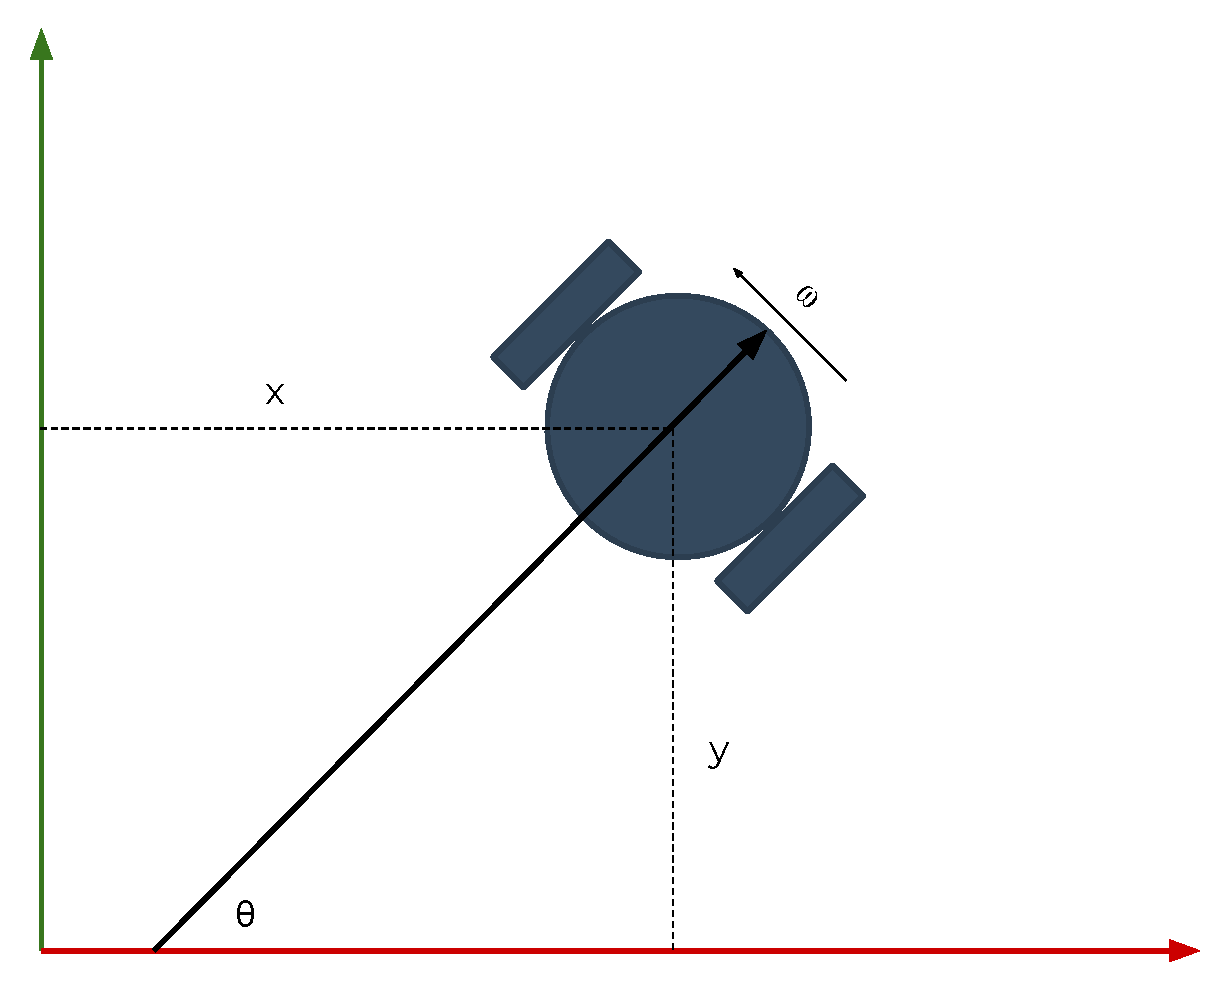
\includegraphics[width=0.8\textwidth]{simulation/figures/odometry.pdf}
    \caption{Robot in local frame \cite{noauthor_16-311_nodate}}
    \label{fig:simulation:odometry_schema}
\end{figure}

As it is a non-linear system of differential equations we can integrate it using a numeric integration.
It can simply be integrated using Euler method expressed in general terms as:
\begin{equation}
    y(t + h) \approx y(t) + h y'(t)
\end{equation}
This method would be computationally cheap, but not as accurate as for example fourth order of Runge-Kutta \cite[p. 40]{noauthor_solving_1993}.
The choice of the method for the numerical integration is mainly based on sample rate we perform with the pi-puck extension.
In the case of e-puck2 physical robot, communication with the on-board \ac{mcu} is configured exchange data with pi-puck extension at around 20Hz.
Considering the slow sample rate and the computational power of the Raspberry Pi Zero to handle floating-point operations, it is reasonable to choose the fourth order of Runge-Kutta over Euler method and trade computation resources for better accuracy.
Therefore, we express the numerical integration as follows:


\begin{equation}
\begin{aligned}
    & k_{00} = v \cos{\theta_{n-1}} \\
    & k_{01} = v \sin{\theta_{n-1}} \\
    & k_{02} = \omega \\
    & \\
    & k_{10} = v \cos{\theta_{n-1} + \frac{t}{2}k_{02}} \\
    & k_{11} = v \sin{\theta_{n-1} + \frac{t}{2}k_{02}} \\
    & k_{12} = \omega \\
    & \\
    & k_{20} = v \cos{\theta_{n-1} + \frac{t}{2}k_{12}} \\
    & k_{21} = v \sin{\theta_{n-1} + \frac{t}{2}k_{12}} \\
    & k_{22} = \omega \\
    & \\
    & k_{30} = v \cos{\theta_{n-1} + t k_{22}} \\
    & k_{31} = v \sin{\theta_{n-1} + t k_{22}} \\
    & k_{32} = \omega
\end{aligned}
\end{equation}

\begin{equation}
\begin{aligned}
    \begin{bmatrix}
        x_n \\
        y_n \\
        \theta_n
    \end{bmatrix} = \begin{bmatrix}
        x_{n-1} \\
        y_{n-1} \\
        \theta_{n-1}
    \end{bmatrix} + \frac{t}{6}
    \begin{bmatrix}
        k_{00} + 2 (k_{10} + k_{20}) + k_{30} \\
        k_{01} + 2 (k_{11} + k_{21}) + k_{31} \\
        k_{02} + 2 (k_{12} + k_{22}) + k_{32}
    \end{bmatrix} 
\end{aligned}
\end{equation}

Notice in Fig. \ref{fig:simulation:odometry} that the orientation is represented as a quaternion while our orientation is represented Euler angles. To convert the Euler angles to quaternions we reference to \cite[p. 12]{diebel_representing_2006}: 

\begin{equation}
    \bm{q}(\alpha_x, \alpha_y, \theta) = \begin{bmatrix}
        \cos{\frac{\alpha_x}{2}} \cos{\frac{\alpha_y}{2}} \cos{\frac{\theta}{2}} + \sin{\frac{\alpha_x}{2}} \sin{\frac{\alpha_y}{2}} \sin{\frac{\theta}{2}} \\
        -\cos{\frac{\alpha_x}{2}} \sin{\frac{\alpha_y}{2}} \sin{\frac{\theta}{2}} + \cos{\frac{\alpha_y}{2}} \cos{\frac{\alpha_y}{2}} \sin{\frac{\theta}{2}} \\
        \cos{\frac{\alpha_x}{2}} \cos{\frac{\theta}{2}} \cos{\frac{\alpha_y}{2}} + \sin{\frac{\alpha_x}{2}} \cos{\frac{\alpha_y}{2}} \sin{\frac{\theta}{2}} \\
        \cos{\frac{\alpha_x}{2}} \cos{\frac{\alpha_y}{2}} \sin{\frac{\theta}{2}} - \sin{\frac{\alpha_x}{2}} \sin{\frac{\theta}{2}} \sin{\frac{\alpha_y}{2}}
    \end{bmatrix}
\end{equation}
in which we can neglect $ \alpha_x $ and $ \alpha_y $ as those two elements are always 0 for differentially-wheeled robots.

At this point, the obtained $ x, y, \bm{q}, \dot{x}, \dot{y} $ and $ \dot{\theta} $ are packed in \texttt{nav\_msgs/Odometry} (see Fig. \ref{fig:simulation:odometry}) and published periodically at 20Hz.

With \texttt{nav\_msgs/Odometry} messages the rest of the \ac{ros2} is aware of robot's odometry data.
However, in addition to odometry data, the odometry frame has to be defined as well to explain the robot's position with respect to the odometry frame.
For that purpose \ac{ros2} defines transform messages of type \texttt{geometry\_msgs/TransformStamped} (see Fig. \ref{fig:simulation:transform}).
In short, transform messages are used to create a transform tree to keep track of multiple coordinate frames over time. 
Keeping track of the coordinate frames is an essential aspect of \ac{ros} in general, and it will be properly explained in Chapter \ref{chap:generalization} in which it will be extensively utilized.

\begin{figure}[H]
    \centering
    \begin{subfigure}[b]{0.9\textwidth}
        \dirtree{%
            .1 geometry\_msgs/TransformStamped.
            .2 (std\_msgs/Header) header.
            .2 (string) child\_frame\_id.
            .2 (geometry\_msgs/Transform) transform.
            .3 (geometry\_msgs/Vector3) translation.
            .3 (geometry\_msgs/Quaternion) rotation.
        }
    \end{subfigure}
    \caption{\texttt{geometry\_msgs/TransformStamped} message type definition in \ac{ros2}}
    \label{fig:simulation:transform}
\end{figure}
However, to control the robot's velocity a message of type \texttt{geometry\_msgs/Twist} (see Fig. \ref{fig:simulation:twist}) has to be utilized.
Therefore, the node has to subscribe to the topic and set the wheels' angular speed accordingly.

\begin{figure}[H]
    \centering
    \begin{subfigure}[b]{0.9\textwidth}
        \dirtree{%
            .1 geometry\_msgs/Twist.
            .2 (std\_msgs/Header) header.
            .2 (geometry\_msgs/Vector3) linear.
            .2 (geometry\_msgs/Vector3) angular.
        }
    \end{subfigure}
    \caption{\texttt{geometry\_msgs/Twist} message type definition in \ac{ros2}}
    \label{fig:simulation:twist}
\end{figure}

The target velocity of the left ($v_{left}$) and right ($v_{right}$) can be obtained as:
\begin{equation}
\begin{aligned}
    & v_{left} = v_{ref} + L \frac{\omega_{ref}}{2} \\
    & v_{right} = v_{ref} - L \frac{\omega_{ref}}{2}
\end{aligned}
\end{equation}
where $ v_{ref}  $ is reference linear velocity (available in the \ac{ros2} message \texttt{.linear.x}) and $ \omega_{ref} $ angular reference velocity (available in the \ac{ros2} message \texttt{.angular.z}). Webots expect the velocity to be given in radians per second (rad/s):
\begin{equation}
\begin{aligned}
    & \omega_{left} = \frac{v_{left}}{R} \\
    & \omega_{right} = \frac{v_{ref}}{R} 
\end{aligned}
\end{equation}

Within this section, a minimal implementation of velocity control and odometry is given.
It allows the e-puck2 to use the standard \ac{ros2} interface to receive velocity control commands and to publish it's position and other relevant information within the odometry frame.
Messages of type \texttt{geometry\_msgs/TransformStamped} are published to topic name \texttt{/tf}, messages of type \texttt{nav\_msgs/Odometry} are published to a topic name \texttt{/odom} and messages of type \texttt{geometry\_msgs/Twist} are received from topic name \texttt{/cmd\_vel}.
Those topic names follow \ac{ros2} conventions for topic naming and can be changed using \ac{ros2} remapping\footnote{Tutorial on \ac{ros2} remapping can be found at \url{https://index.ros.org/doc/ros2/Tutorials/Node-arguments/\#id1}.}. 

\subsection{Distance Sensors}
E-puck2 is equipped with 8 infra-red sensors and one \ac{tof} sensor (see Fig. \ref{fig:simulation:distance_sensors}). These sensors are modeled as \texttt{DistanceSensor}\footnote{More information about \texttt{DistanceSensor} nodes is available \url{https://cyberbotics.com/doc/reference/distancesensor}.} in Webots.

\begin{figure}[H]
    \centering
    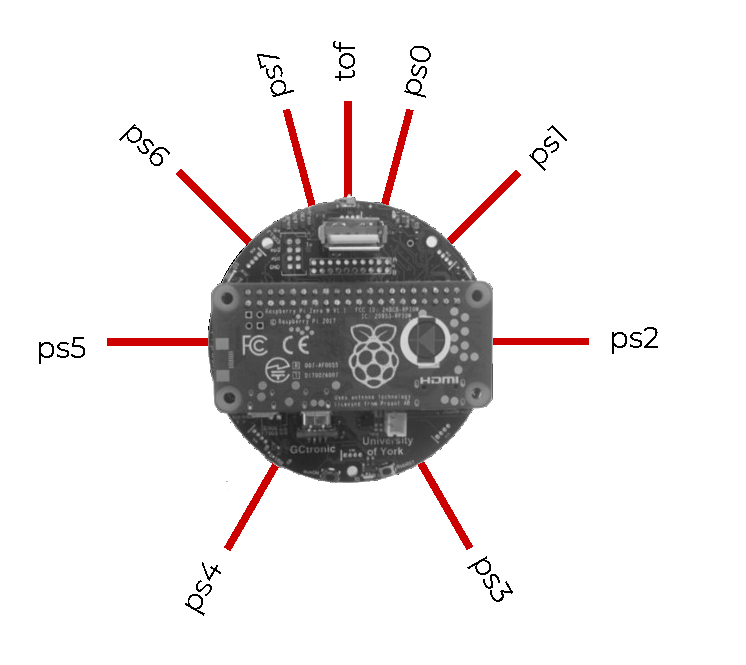
\includegraphics[width=0.65\textwidth]{simulation/figures/distance_sensors.pdf}
    \caption{Distance sensors available on e-puck2}
    \label{fig:simulation:distance_sensors}
\end{figure}

All details about the sensors are obtained from the Webots and published to a topic of type \texttt{sensor\_msgs/Range}\footnote{Definition of \texttt{sensor\_msgs/Range} message type is available at \url{https://github.com/ros2/common_interfaces/blob/master/sensor_msgs/msg/Range.msg}.}.

\subsubsection{Laser Scanner}
\ac{ros2} defines \texttt{sensor\_msgs/LaserScan}\footnote{Definition of \texttt{sensor\_msgs/LaserScan} message type is available at \url{https://github.com/ros2/common_interfaces/blob/master/sensor_msgs/msg/LaserScan.msg}.} for \acp{lidar} and other types of planar laser range-finders.
Those messages are commonly used by \ac{ros2} community packages like \texttt{navigation2} and \texttt{slam\_toolbox}.
The message type requires an array of measurements at angles that are equally distanced from each other. 

Therefore, even though there is no \ac{lidar} available on the e-puck2 it is possible to emulate it using available distance sensors.
Since the distance sensors are not evenly distributed, virtual distance sensors are added to fill space between the actual distance sensors (see Fig. \ref{fig:simulation:laserscan}).
These virtual distance sensors always give measurements of 0 meters which corresponds to invalid measurement (as minimum valid range in \texttt{sensor\_msgs/LaserScan} message is defined to be greater than 0 meters).
% TODO: Explain https://answers.ros.org/upfiles/14177210732958238.jpg

\begin{figure}[H]
    \centering
    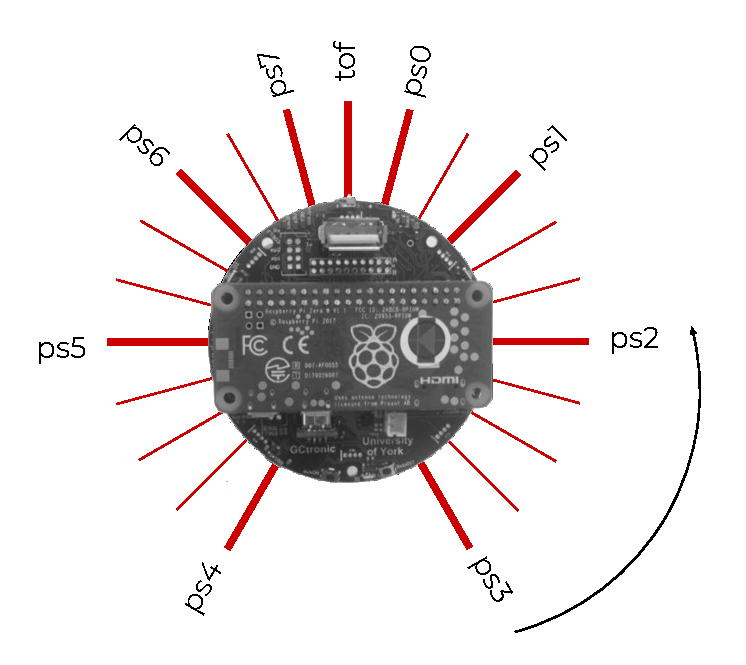
\includegraphics[width=0.8\textwidth]{simulation/figures/laserscan.pdf}
    \caption{Virtual distance sensors are added to emulate \ac{lidar}, making the angle difference between the rays constant ($15^\circ$)}
    \label{fig:simulation:laserscan}
\end{figure}

\subsection{Light Sensors}
E-puck2 has eight infra-red sensors which besides proximity can measure light intensity as well.
\ac{ros2} interface for light sensors uses messages of type \texttt{sensor\_msgs/Illuminance}\footnote{Definition of \texttt{sensor\_msgs/Illuminance} message type is available at \url{https://github.com/ros2/common_interfaces/blob/master/sensor_msgs/msg/Illuminance.msg}.}.
The message type requires the measurements to be in Lux units (illuminance) while measurements acquired in Webots\footnote{Light sensors in Webots are represented as \texttt{LightSensor} node - \url{https://cyberbotics.com/doc/reference/lightsensor}.} are expressed in watts per square meter [$W/m^2$] (irradiance). 
The conversion is done according to \cite{michael_conversion_2019}.

\subsection{\acl{imu}}
\ac{imu} in Webots modeled as two nodes, \texttt{Accelerometer} and \texttt{Gyro}.
Measurements from those two nodes are combined and packed into messages of type \texttt{sensor\_msgs/Imu}.

\subsection{Camera}
Typically, cameras in \ac{ros2} use two topics, one for data (images) and another one for intrinsic camera parameters.
Images from Webots camera node are sampled, packed in \ac{ros2} messages of type \texttt{sensor\_msgs/Image} and published repeatedly.
The intrinsic parameters are defined by \ac{ros2} has the following form:
\begin{equation}
K = \begin{bmatrix}
    f_x & 0 & c_x \\
    0 & f_y & c_y \\
    0 & 0 & 1
\end{bmatrix}
\end{equation}

Webots doesn't provide such a matrix, but it is straightforward to create one from the existing parameters.
Since Webots camera doesn't provide distortions that move the focal length then $f_x = f_y$ which is equal to the focal length that can be obtained in Webots (e.g. \texttt{getFocalLength()}).
The principal point also doesn't have offset, but it is in the center of the image $c_x$ is equal to $ \frac{\texttt{image\_width}}{2} $ and $c_y$ is equal to $ \frac{\texttt{image\_height}}{2} $.

\subsection{\acsp{led}}
There are eight \acsp{led} available in the robot and they are controlled with messages of type \texttt{std\_msgs/Int32}.
The last three bytes of the value are used to set three \ac{rgb} components in case of \acsp{rgbled} and for the regular \acp{led} the value is used to set the intensity.
Arguably here, message type \texttt{std\_msgs/ColorRGBA} may be more suitable, but \texttt{std\_msgs/Int32} is chosen to be more consistent with Webots \ac{api}.

\subsection{Final Interface}

In the table bellow (see Table \ref{tab:simulation:complete_interface}) the final interface is shown.

\begin{table}[H]
    \begin{adjustwidth}{-1.5in}{-1.5in}
    \centering
    \begin{tabular}{|l|l|l|}
        \hline
        \textbf{Topic name} & \textbf{Message type} & \textbf{Description} \\
        \hline
        \texttt{/cmd\_vel} & \texttt{geometry\_msgs/Twist} & Controls robot's velocity \\
        \hline
        \texttt{/odom} & \texttt{nav\_msgs/Odometry} & Odometry measurements from wheels \\
        \hline
        \texttt{/ps[0-7]} & \texttt{sensor\_msgs/Range} & Measurements from infra-red sensors \\
        \hline
        \texttt{/tof} & \texttt{sensor\_msgs/Range} & Measurements from \acs{tof} sensor \\
        \hline
        \texttt{/scan} & \texttt{sensor\_msgs/LaserScan} & Emulated \ac{lidar} measurements \\
        \hline
        \texttt{/ls[0-7]} & \texttt{sensor\_msgs/Illuminance} & Light measurements from infra-red sensors \\
        \hline
        \texttt{/imu} & \texttt{sensor\_msgs/Imu} & Measurements from \acs{imu} \\
        \hline
        \texttt{/led[0-7]} & \texttt{std\_msgs/Int32} & Controls \acsp{led} \\
        \hline
        \texttt{/gs[0-2]} & \texttt{sensor\_msgs/Range} & Measurements from ground sensors \\
        \hline
        \texttt{/image\_raw} & \texttt{sensor\_msgs/Image} & Camera images \\
        \hline
        \texttt{/camera\_info} & \texttt{sensor\_msgs/CameraInfo} & Camera intrinsic parameters \\
        \hline
        \texttt{/tf} & \texttt{tf2\_msgs/TFMessage} & Dynamic transforms \\
        \hline
        \texttt{/tf\_static} & \texttt{tf2\_msgs/TFMessage} & Static transforms \\
        \hline
    \end{tabular}
    \caption{Complete \ac{ros2} interface for e-puck2 robot}
    \label{tab:simulation:complete_interface}
    \end{adjustwidth}
\end{table}

In addition to the previously mentioned topics, there are topics with name \texttt{/gs[0-2]}, and those topics publish data from ground sensors.
The ground sensors can be bought as a separate e-puck2 module.
Therefore, this part of the \ac{ros2} interface will be automatically created if the module is present in the e-puck.

Another topic not mentioned before is \texttt{/tf\_static}. 
It is used to describe transformations between different coordinate frames that do not typically change (for example, a transformation between the robot's base and the \ac{lidar}).
Messages published to this topic have specific \ac{qos} configured, durability is set to be transient local.
The transient local \ac{qos} means that the nodes joined to the system will receive the messages even though the messages are published much earlier and avoiding periodic publishing reduces the load on the \ac{ros2} driver as the messages have to be published only once.

Another performance improvement is made by not publishing the messages all the time. Messages are published only if the subscribers are available.
This significantly improves performance, especially in the camera's case, as it is very \acs{cpu}/\acs{gpu} intensive task.
For example, on the same computer and in the same Webots simulation, with camera of resolution 640x480, the simulation can run almost 2 times faster (1.81 times faster in e-puck2 default word).
The difference can be much bigger for robots with multiple camera and many other sensors.

\note{---------------I have to stop here for a moment...}
% TODO: Continious Integration
}{}
\iftoggle{FULL_REPORT}{\chapter{\acs{ros2} Interface for Physical E-puck2}
\label{chap:physical}
\shorttitle{\nameref{chap:physical}}

Details about \ac{ros2} interface implementation on e-puck2 physical robot will be given in this chapter.
Even though the objective is to create the same \ac{ros2} interface as one explained in the previous chapter the implementation is very different.
The difference mostly comes from the physical interface to the sensors and actuators, performance limitations, and \ac{cpu} architecture.
Therefore, these differences will be emphasized in this chapter.

\section{Introduction}

Pi-puck extension uses \ac{i2c} and \ac{usb} to communicate with sensors and actuators available on the e-puck2 robot (see Fig. \ref{fig:physical:general}).

\begin{figure}[H]
    \centering
    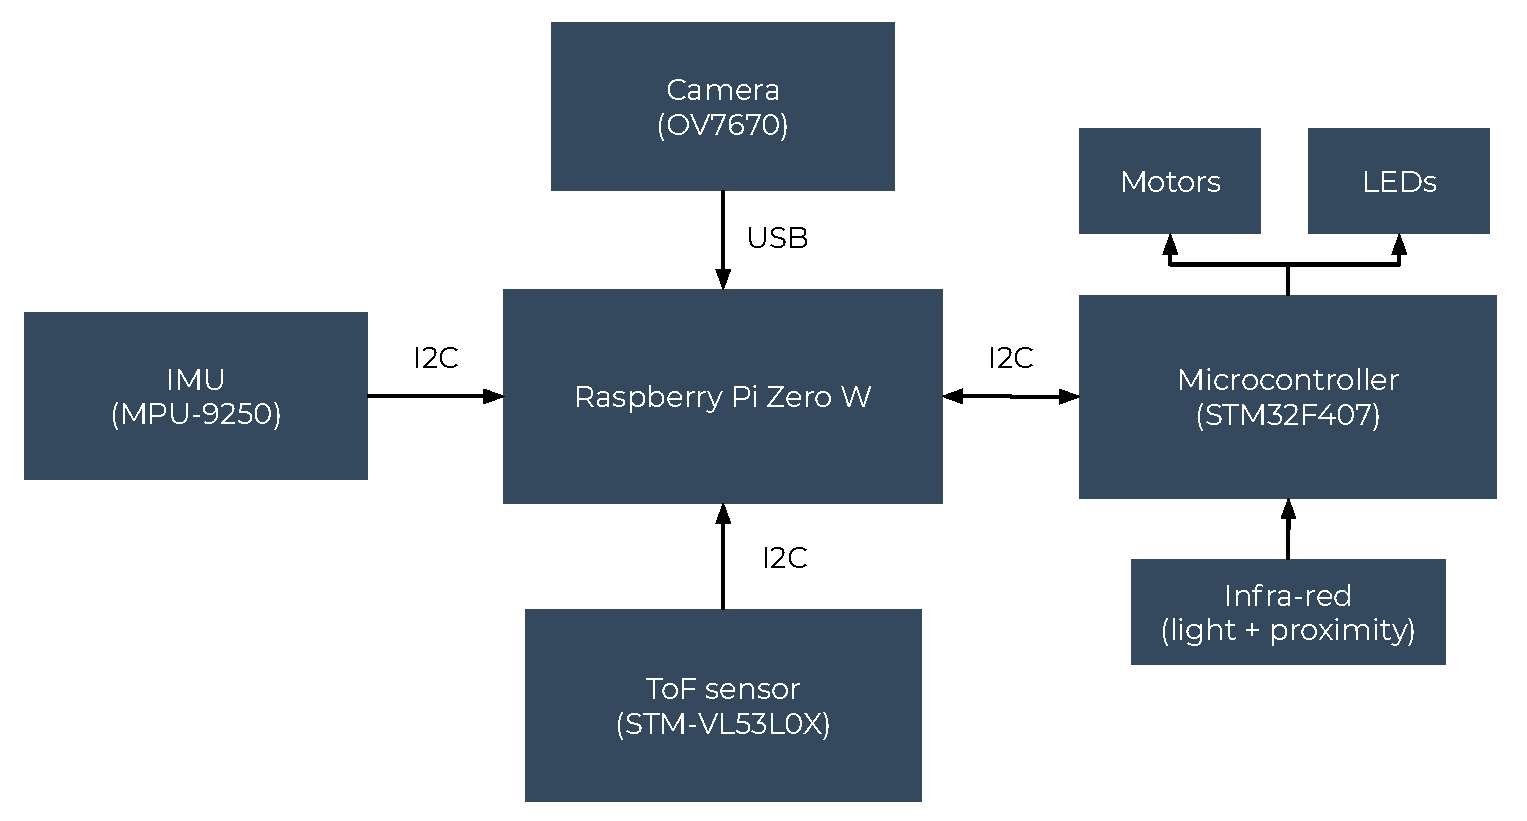
\includegraphics[width=\textwidth]{physical/figures/general.pdf}
    \caption{Components utilized in \ac{ros2} driver}
    \label{fig:physical:general}
\end{figure}

In case \acp{led}, motors, and infrared sensors the communication is done through on-board \ac{mcu}.
In the case of infrared sensors, this is necessary as Raspberry Pi Zero W doesn't have any \ac{dac} module. 
Therefore, the \ac{mcu} acts as a slave that stands between analog sensors and actuators, or actuators that require deterministic updates (motors).
With \ac{imu} and the \ac{tof} sensor, Raspberry Pi Zero Zero W communicates directly over \ac{i2c}, while with the camera the communication is done over \ac{usb}. 

\begin{table}[H]
    \centering
    \begin{tabular}{|l|l|}
        \hline
        \textbf{Sensor function} & \textbf{Sensor model} \\
        \hline
        Camera & Omnivision OV7670 CMOS\footnote{Datasheet of the OV7670 sensor is available at \url{http://projects.gctronic.com/epuck2/doc/OV7670.pdf}.} \\
        \hline
        Distance and light sensors & TCRT1000 \\
        \hline
        \ac{imu} & InvenSense MPU-9250 \\
        \hline
        \ac{tof} & STM-VL53L0X \cite{lakovic_application_2019} \\
        \hline
    \end{tabular}
    \caption{List of the relevant sensors available on e-puck2 robot shown in Fig. \ref{fig:physical:general}}
    \label{tab:physical:sensors}
\end{table}

The protocol used to communicate with the sensors is explained in the corresponding sensor's documentation, while the communication with the \ac{mcu} is specified by the format shown in Table \ref{tab:physical:rpi_to_mcu} and Table \ref{tab:physical:mcu_to_rpi}.

\begin{table}[H]
    \centering
    \begin{tabular}{c|c|c|c}
    \hline
    \textbf{Left speed (2)} & Right speed (2) & Speaker (1) & LED[1,3,5,7] (1)  \\
    \hline
    LED2 (3) & LED4 (3) & LED6 (3) & LED8 (3) \\
    \hline
    Settings (1) & \textbf{Checksum (1)} & & \\
    \hline
    \end{tabular}
    \caption[Message format sent from the Raspberry Pi Zero W to the \ac{mcu}]{Message format sent from the Raspberry Pi Zero W to the \ac{mcu}. Bolded fields highlight the most and the least significant bytes in the packet.}
    \label{tab:physical:rpi_to_mcu}
\end{table}

\begin{table}[H]
    \centering
    \begin{tabular}{c|c|c|c}
    \hline
    \textbf{8 x Prox (16)} & 8 x Ambient (16) & 4 x Mic (8) & Selector + button (1) \\
    \hline
    Left steps (2) & Right steps (2) & TV remote (1) & \textbf{Checksum} \\
    \hline
    \end{tabular}
    \caption[Message format sent from the \ac{mcu} to the Raspberry Pi Zero W]{Message format sent from the \ac{mcu} to the Raspberry Pi Zero W. Bolded fields highlight the most and the least significant bytes in the packet.}
    \label{tab:physical:mcu_to_rpi}
\end{table}

\section{\ac{ros2} on Raspberry Pi OS}
Before \ac{ros2} driver is created \ac{ros2} has to be installed on the Raspberry Pi Zero W.
The board comes with \ac{cpu} with arm32 architecture and Raspberry Pi OS.
This configuration is not officially supported by \ac{ros2} and standard installation procedure using \acs{os}' package manager doesn't work.
The closest official support is a source compilation for Debian Buster placed as a tier 3 support\footnote{\ac{ros2} supported platforms are defined by REP 2000 available at \url{https://www.ros.org/reps/rep-2000.html\#foxy-fitzroy-may-2020-may-2023}.}.
This means that \ac{ros2} has to be cross-compiled and that potential incompatibilities have to be manually resolved.

Since the \ac{ros2} driver is intended for a wide range of users the installation procedure has to be user-friendly.
In that purpose, three user guides are created to simplify the installation procedure, using pre-configured \ac{sdcard}, compilation on Raspberry Pi Zero W, and cross-compilation from the user's \ac{pc}.
A comparison of these methods is given by Table \ref{tab:physical:installation}.

\begin{table}[H]
    \begin{adjustwidth}{-1.5in}{-1.5in}
    \centering
    \begin{tabular}{|l|c|c|c|}
        \hline
        & \textbf{Using image} & \textbf{Compilation on the board} & \textbf{Cross-compilation} \\
        \hline
        Compilation speed & ++ & - & + \\
        \hline
        Easy to use & ++ & - & -- \\
        \hline
        Flexibility & -- & ++ & + \\
        \hline
    \end{tabular}
    \caption{Comparison of different installation methods provided in the scope of the project}
    \label{tab:physical:installation}
    \end{adjustwidth}
\end{table}

Using the existing image with \ac{ros2} and other tools configured is the easiest approach for the users.
The problem appears once the user has to upgrade the \ac{ros2} version, install a new package, or to develop a custom package that has a lot of dependencies as compilation time is slow.
For those use cases, cross-compilation tools are provided.

\subsection{\ac{ros2} Cross-compilation}
In the scope of the project, tools are built to help with the process of \ac{ros2} cross-compilation.
All cross-compilation dependencies and configurations are packaged into a Docker container\footnote{Thorough guide about the \ac{ros2} cross-compilation is available at \url{https://github.com/cyberbotics/epuck_ros2/tree/master/installation/cross_compile}.}.
This means that the user doesn't need to worry about host \ac{os} and tools compatibility. 

\begin{figure}[H]
    \centering
    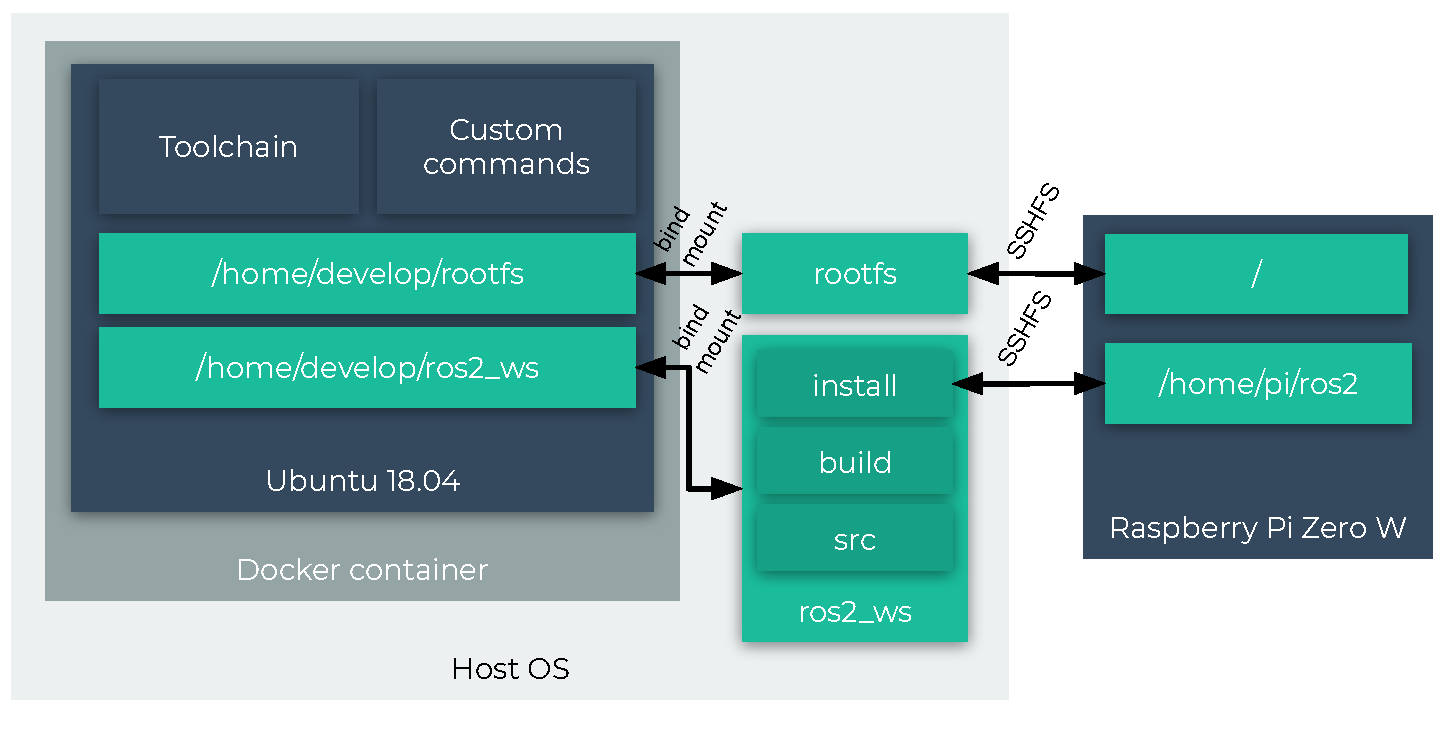
\includegraphics[width=\textwidth]{physical/figures/cross_compilation.pdf}
    \caption{\ac{ros2} cross-compilation setup}
    \label{fig:physical:cross_compilation}
\end{figure}

The typical setup of using the cross-compilation tools built within this project is shown in Fig. \ref{fig:physical:cross_compilation}.
Boxes in green represent directories while the others are software tools.
\texttt{ros2\_ws} is \ac{ros2} workspace, it contains source files, temporary build files and compiled output, libraries and executable.
The source code available in this directory is compiled with cross-compilation tools in the Docker container while the result stays available on the host \ac{os}.
To build certain packages, compilers need filesystem of the Raspberry Pi Zero W (\texttt{rootfs}) to compile and link dependencies available on the board.
Both directories are available in the Docker container as well as on the host \ac{os}.

Once the \ac{ros2} packages are compiled they can be used by copying \texttt{ros\_ws/install} directory or by mounting it to the Raspberry Pi Zero W.
Although, mounting the directory can significantly increase the productivity as the process of copying the files can be avoided.

% TODO: Typical errors

\section{Programming Language}
Initially, \ac{ros2} driver, with a few basic features, for the physical e-puck2 is implemented in Python programming language.
However, as the \ac{ros2} driver included more sensors the \ac{cpu} load was too high to handle other functionalities. 

\begin{figure}[H]
\centering
\begin{subfigure}{.8\textwidth}
  \centering
  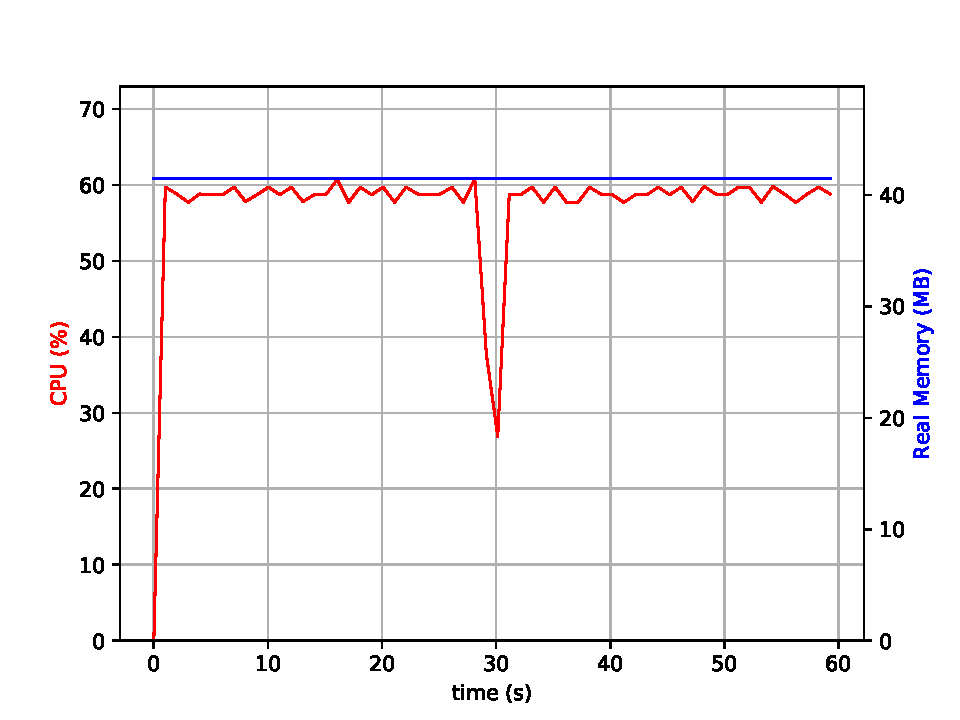
\includegraphics[width=\linewidth]{physical/figures/rpi_py_32ms}
  \caption{\ac{cpu} and \ac{ram} load with Python}
  \label{fig:physical:py_vs_cpp:py}
\end{subfigure}
\begin{subfigure}{.8\textwidth}
  \centering
  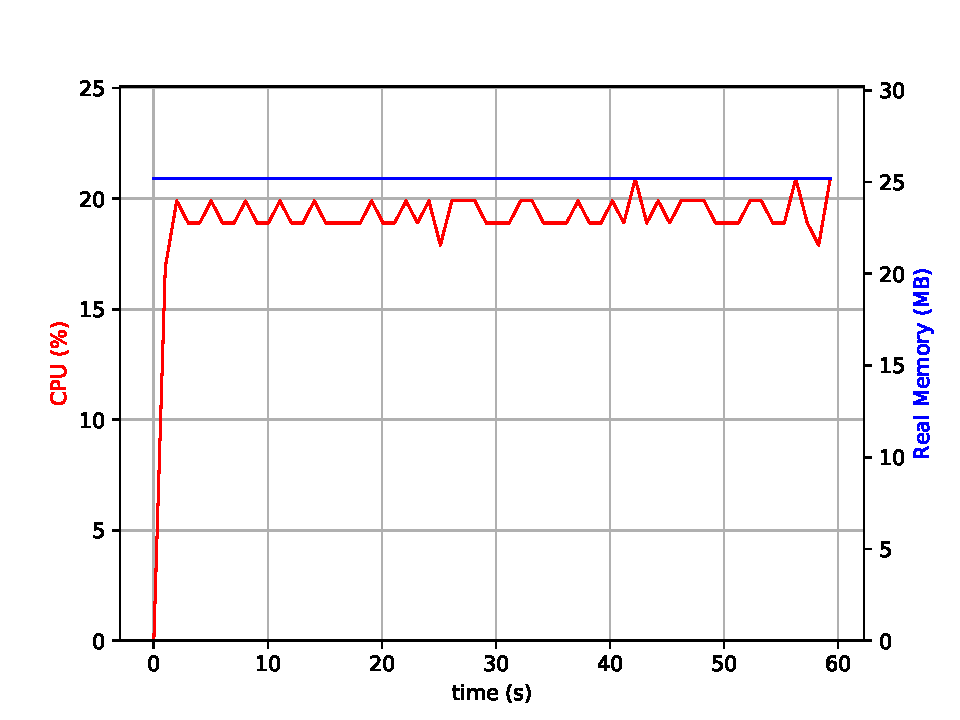
\includegraphics[width=\linewidth]{physical/figures/rpi_cpp_32ms}
  \caption{\ac{cpu} and \ac{ram} load with C++}
  \label{fig:physical:py_vs_cpp:cpp}
\end{subfigure}
\caption[Performance comparison of implementations in Python and C++]{Performance comparison of the similar node \ac{ros2} node implemented in Python and C++. The \ac{cpu} and \ac{ram} load is measured using \texttt{psrecord} tool\footnotemark}
\label{fig:physical:py_vs_cpp}
\end{figure}
\footnotetext{The exact command to measure the load is \texttt{psrecord \$(pgrep epuck2\_driver) --interval 1 --plot plot.pdf --duration 60}}

In Fig. \ref{fig:physical:py_vs_cpp} performances of Python and C++ implementation of similarly implemented \ac{ros2} node that provide the same functionalities are given.
More precisely, they both publish odometry data, measurements from eight distance sensors, laser scan, and they are both subscribed to the velocity control topic.
In the figure, we can observe that \ac{cpu} usage is three times lower while \ac{ram} is almost two times lower.
This analysis in early stage of implementation steered the development towards C++\footnote{One of the bottlenecks was in \ac{ros2} client library for Python (\texttt{rclpy}) related to timer implementation - \url{https://github.com/ros2/rclpy/issues/520}. Fixing it improved the performances, but C++ implementation was still more efficient.}.

\section{Camera}
As mentioned before, the camera available on e-puck2 (Omnivision OV7670 CMOS) captures images at 15 \acs{fps} in resolution of 640x480.
Compared to the simulation, data produced by the camera has to be efficiently processed and intrinsic camera parameters have to be determined.

\subsection{Camera Optimization}
Our preliminary investigation showed that the \ac{ros2} driver wasn't able to publish images more frequently than 3-4 \acs{fps} (thorough analysis is available in Chapter \ref{chap:results}).
Publishing raw (uncompressed) images would cause the network to become a bottleneck while compressing the images before transmitting would put a high \ac{cpu} load, effectively limiting \ac{fps}.
Fortunately, there is \ac{gpu} available on Raspberry Pi Zero W on which certain image manipulation tasks can be offloaded.

\subsubsection{Introduction}
A brief overview on \ac{gpu} on Raspberry Pi Zero W will be given first. Typical architecture of the \ac{gpu} and the related components is given by the following figure (Fig. \ref{fig:physical:gpu_architecture}):
 
 \begin{figure}[H]
    \centering
    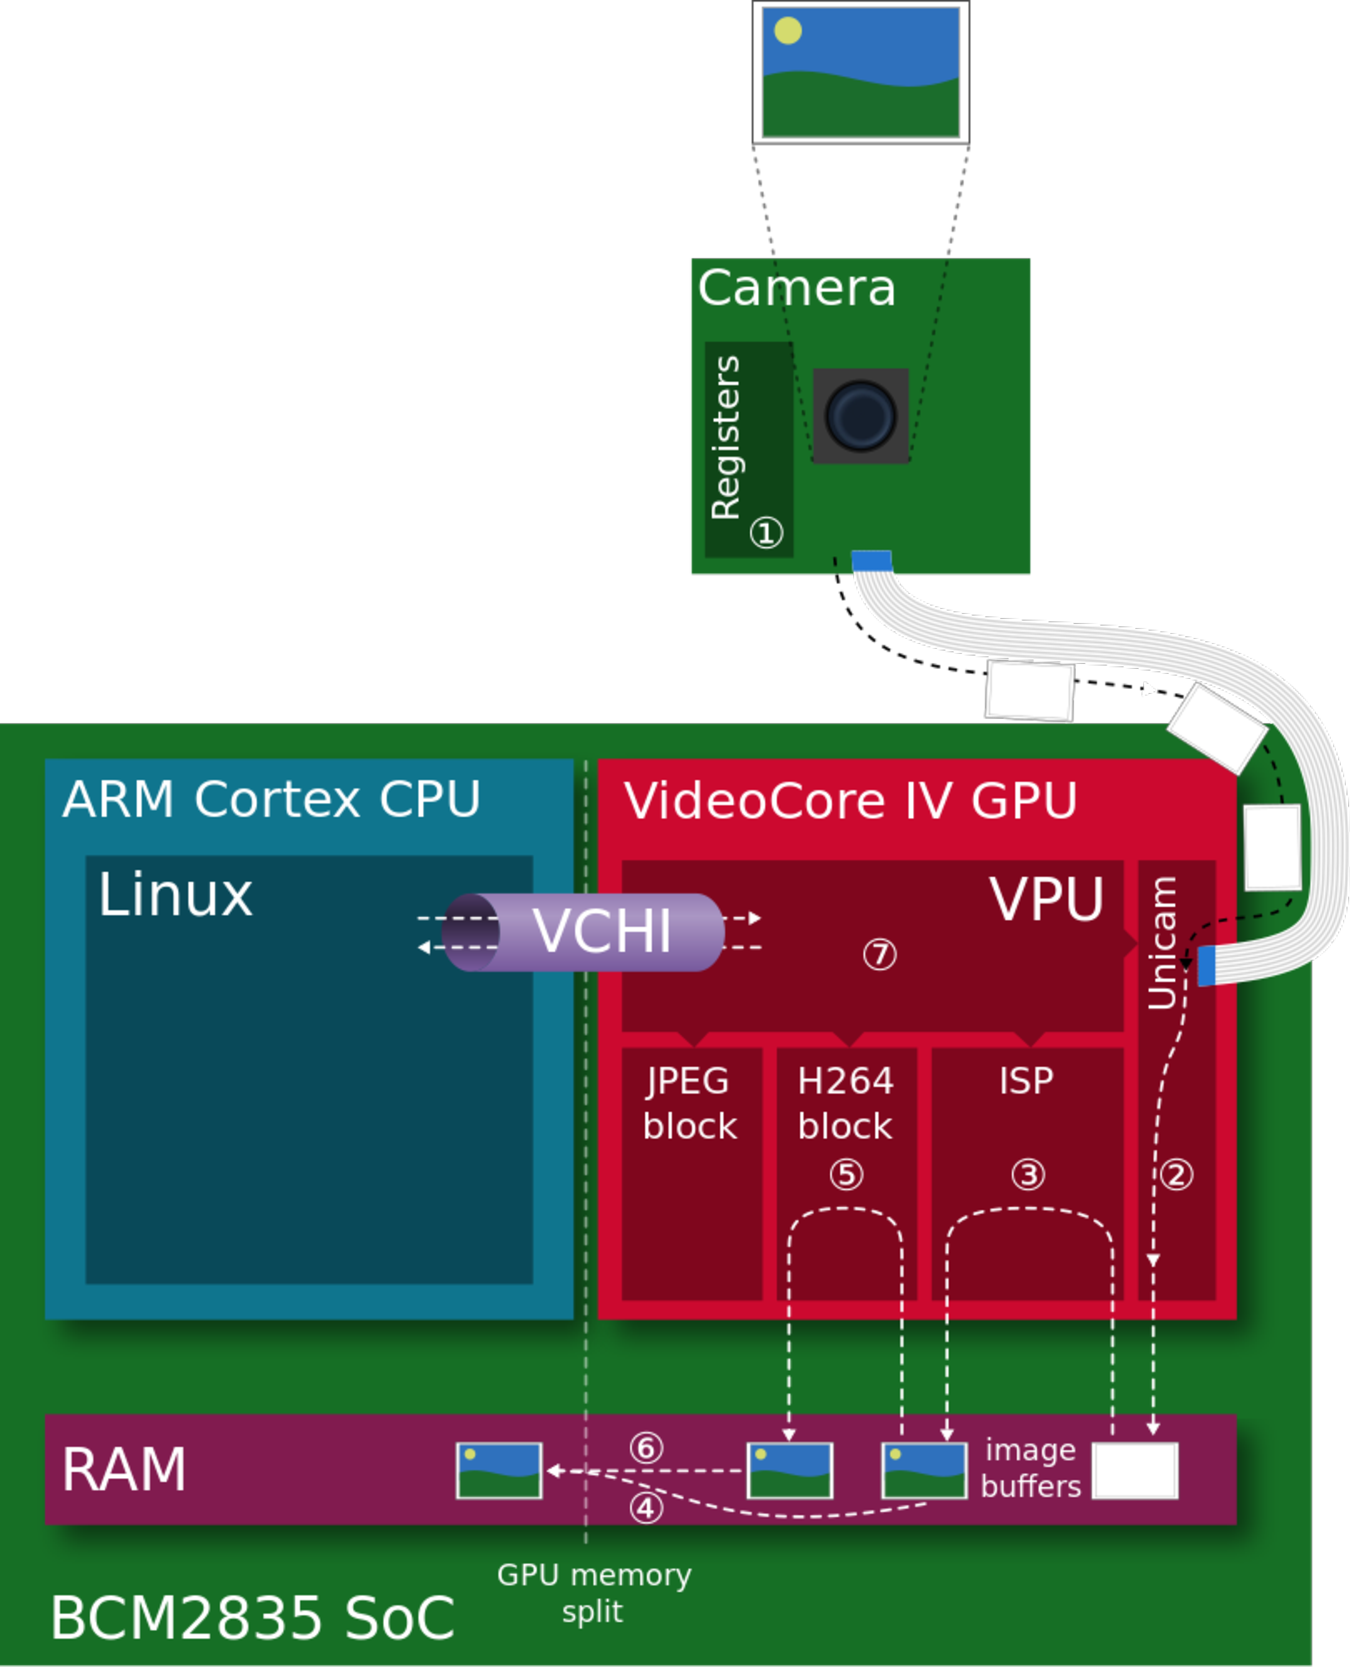
\includegraphics[width=0.8\textwidth]{physical/figures/gpu_architecture}
    \caption{\ac{gpu} architecture \cite{noauthor_videocore_nodate-1}}
    \label{fig:physical:gpu_architecture}
\end{figure}

In the figure, there are three main components on the \ac{soc}, \ac{cpu}, \ac{gpu} and \ac{ram}.
Further, \ac{gpu} has it's own computational components dedicated for different image processing tasks.
These components are orchestrated by \ac{vcos} (abstraction layer on top of an \ac{rtos}) which also reads images from the camera.
Signaling between \ac{cpu} and \ac{gpu} is done through \ac{vchi} while the images are shared by storing them on \ac{ram}.
From the software point of view, \ac{mmal} library is used to interact with the \ac{gpu}.
The library is based on \ac{omx} and the goal is to ensure consistent interface across all \acp{gpu} available in different models of Raspberry Pi.
For comprehensive explanation about hardware blocks read \cite{noauthor_videocore_nodate-1} and for software \cite{noauthor_videocore_nodate}, both are great sources of information.

\subsubsection{\ac{ros2} Camera Driver Implementation}
There are a few available \ac{ros1} and \ac{ros2} packages that implement \ac{gpu} accelerated image acquisition and processing.
Unfortunately, these packages expect the camera to be connected via \ac{csi} which is not the case in e-puck2. 
Therefore, the whole \ac{ros2} camera node is implemented from scratch, including image acquisition based on \ac{v4l2} and image processing (compression and resizing) based on \ac{mmal}.
 
 \begin{figure}[H]
    \centering
    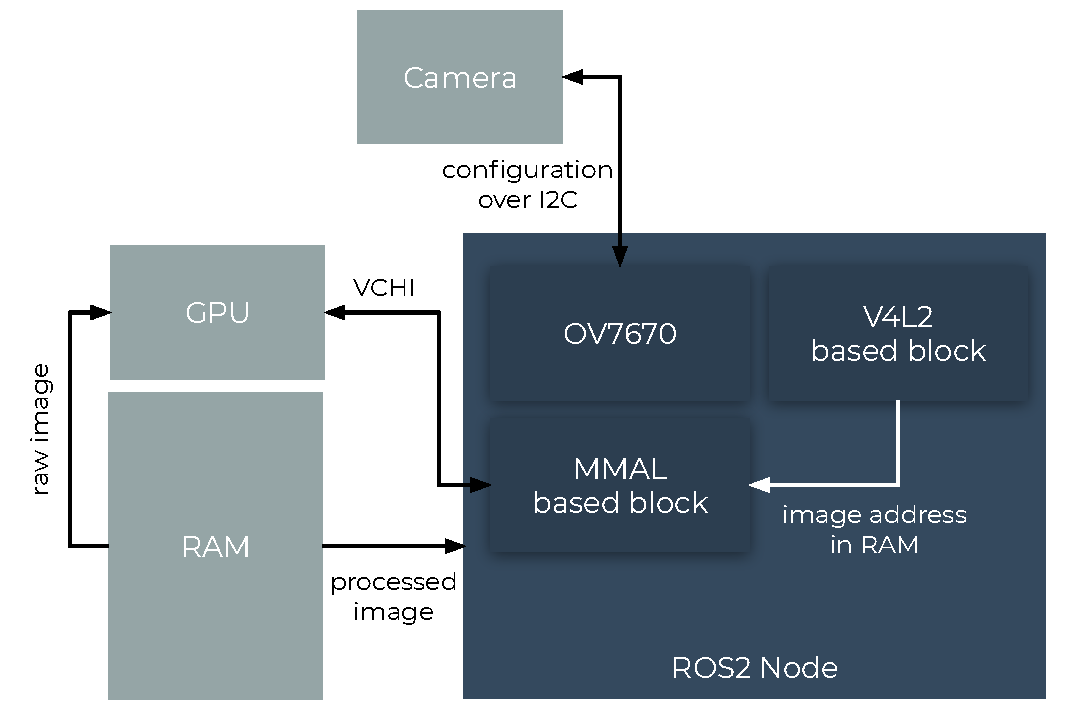
\includegraphics[width=0.8\textwidth]{physical/figures/camera_software_architecture.pdf}
    \caption{Camera software architecture}
    \label{fig:physical:camera_software_architecture}
\end{figure}
 
 In Fig. \ref{fig:physical:camera_software_architecture} a software architecture of the camera node is given. 
 Initially, the camera is configured over \ac{i2c} (block \texttt{OV7670}) and then \ac{v4l2} is used to initiate image capture and store it to the \ac{ram}.
 The pointer to the image is passed through \ac{mmal} block which interacts with \ac{gpu} to compress and resize it. 
 Finally, \ac{gpu} stores the processed image to the \ac{ram} and the pointer the processed image is available to the \ac{ros2} camera node.
 The node packs it into the corresponding messages type and publishes it.
 
 \subsubsection{\ac{ros2} Camera Driver Usage}
 Since the camera transmits the images through the network compressed they have to be uncompressed once the target computer is reached.
 
\begin{figure}[H]
    \centering
    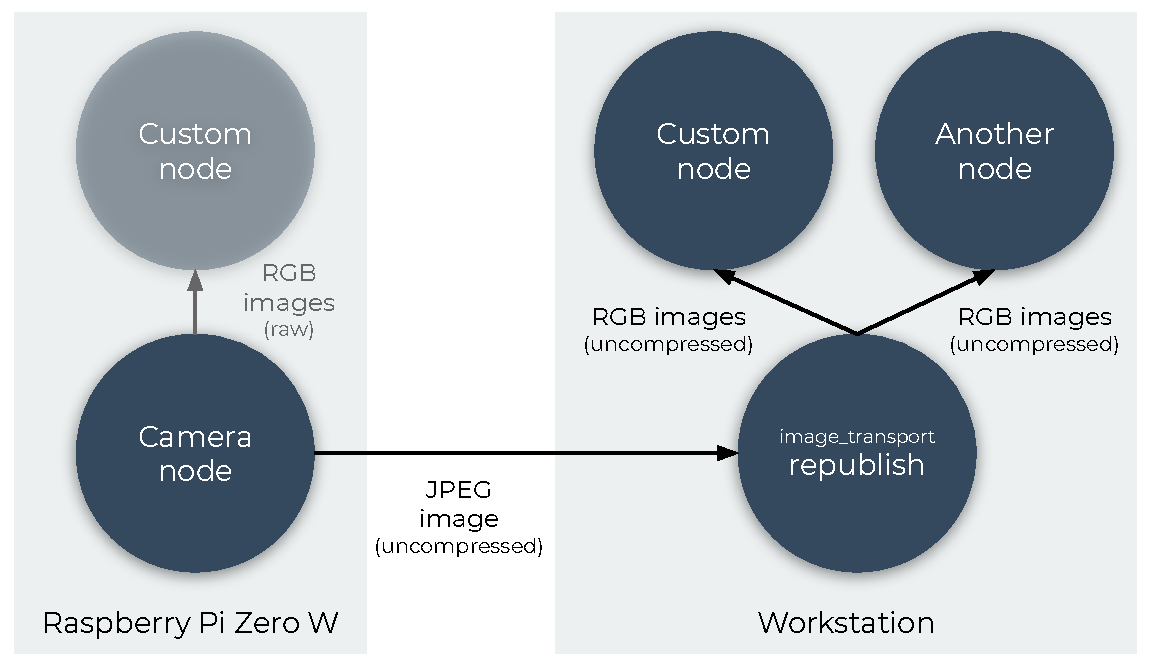
\includegraphics[width=0.8\textwidth]{physical/figures/camera_ros_images.pdf}
    \caption{Image flow within \ac{ros2} application}
    \label{fig:physical:camera_ros_images}
\end{figure}

Fig. \ref{fig:physical:camera_ros_images} shows typical flow of images within \ac{ros2} application.
The camera node will publish \acs{rgb} or \acs{jpeg} compressed images depending on which topic a user is subscribed to.
From the user's perspective \ac{rgb} images desired as pixel-wise operations can be done directly, without decompression.
Therefore, if a user has a custom node running on the Raspberry Pi Zero W the user should subscribe to \ac{rgb} images.
Otherwise, if the user wants to use on the workstation the user should run \texttt{image\_transport/republish} node besides.
The node decompresses the images on the workstation and publishes \ac{rgb} to all local nodes.
This way, a custom node by the user will not change and the only additional action that the user has to do if working on the workstation is running \texttt{image\_transport/republish} node.
 
\subsubsection{Camera Calibration}
In comparison with \ac{ros2} node for the simulated robot intrinsic parameters of the Omnivision OV7670 camera are not known.
These parameters can be found through a calibration process. The process consists of capturing many images, which is known as the physical position of points, and then performing non-linear optimization to find parameters that project these points from the 3D world to 2D plane \cite{lukic_dual_nodate}. This process is automated by creating a custom \ac{ros2} node that relies on OpenCV's calibration module.

\subsection{Differential Drive}
Besides the performance limitations of the Raspberry Pi Zero W that cause issues, there are other limitations as well. In the case of odometry, in Table \ref{tab:physical:rpi_to_mcu}, you can notice that number of ticks for left and the right wheel is limited to 2 bytes. Taking into account it is a signed number (can take a value from -32767 to 32767) and that there are 1000 ticks per revolution it can make around 32 revolutions before overflow (or $ 2 \pi R \frac{32767}{1000} = 4.11m $). This means that the robot's odometry will become completely wrong after around 4 meters. To avoid this, the following simple approach is applied:

\vspace*{.4cm}
\begin{algorithm}[H]
\SetKwInOut{Input}{input}
\SetKwInOut{Output}{output}
\Input{%
    $\bm{N_{overflow}}$ -- Number of overflows (it can be negative) \newline 
    $\bm{N_{grace}}$ -- Constant which represents the maximum difference in number of ticks between two sequential samples \newline 
    $\bm{P_{ticks}}$ -- Number of ticks in the previous sample \newline 
    $\bm{C_{ticks}}$ -- Number of ticks received from the sensor
}
\Output{%
    $\bm{T_{ticks}}$ -- Total (corrected) number of ticks
}

\If{$ |P_{ticks} - C_{ticks}|> 2^{15} - N_{grace} $}{
    \eIf{$P_{ticks} > 0 \land C_{ticks} < 0$}{
        increment $N_{overflow}$\;
    }{
        decrement $N_{overflow}$\;
    }
}
$ T_{ticks} \leftarrow 2^{16} N_{overflow} + C_{ticks} $\;

\caption{Overflow protection algorithm}
\label{alg:physical:overflow}
\end{algorithm}
\vspace*{.4cm}

By applying Alg. \ref{alg:physical:overflow}, in $ T_{ticks} $ a total number of ticks will be stored, taking overflows into the consideration. It is important set $ N_{grace} $ reasonably big such that $ |P_{ticks} - C_{ticks}| > N_{grace} $ is only satisfied when the overflow occurs.

\section{Software Quality Assurance}
As a part of ROSIN\footnote{Software Quality Assurance propositions of ROSIN project can be fount at \url{https://www.rosin-project.eu/software-quality-assurance}.}, this master project has to incorporate software engineering best practices such as continuous integration \cite{meyer_continuous_2014}, unit testing and code reviews. Those practices are fully utilized throughout the whole project and they will be briefly explained here.

\subsection{\ac{ros2} Node Unit Tests}

The unit tests are implemented according to the standard procedure recommended by \ac{ros2}. Two \ac{ros2} nodes are executed, one node is the actual node we want to test while the other one simulates the rest of the application and executes tests. 

\begin{figure}[H]
    \centering
    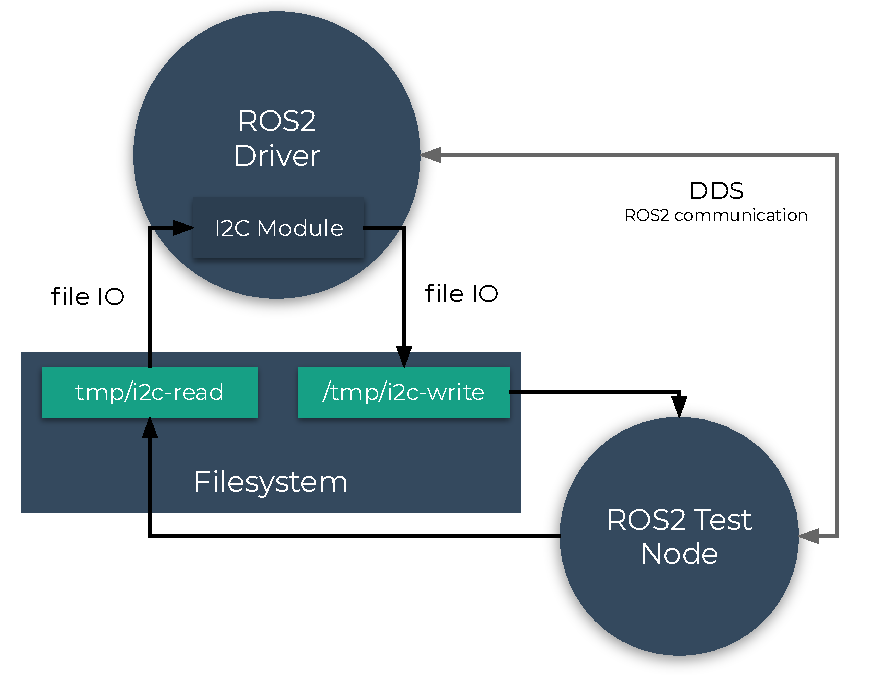
\includegraphics[width=0.8\textwidth]{physical/figures/mocking.pdf}
    \caption{Testing communication with the microcontroller}
    \label{fig:physical:mocking}
\end{figure}

A concrete example for testing of the \ac{ros2} driver is given in Fig. \ref{fig:physical:mocking}. In the figure, \ac{ros2} test node is used to emulate the rest of the \ac{ros2} application. For example, it can publish a message to \texttt{/cmd\_vel} and set angular velocity.
The \ac{ros2} driver should receive the message and send corresponding motor velocity through \ac{i2c}. To verify whether proper commands are sent over \ac{i2c} a special \ac{i2c} module is created.
It implements two modes, in regular mode it interacts with \ac{i2c} directly while in testing, it writes everything to the filesystem. 
This way, \ac{ros2} test node has an opportunity to test commands addressed to the \ac{i2c}.

All unit tests are based on Python's standard unit testing framework \texttt{unittest} and \ac{ros}' \texttt{launch\_test}.

\subsection{Code Quality Tests}
Besides the unit tests, many tests for static code analysis are used as well.
The following tests are used to perform code quality analysis:
\begin{itemize}
    \item \texttt{cppcheck} detects undefined behavior (e.g. dead pointers, division by zero or integer overflows) and security issues (e.g. buffer errors and information leaks) in C++ code.
    \item \texttt{cpplint} verifies whether the user follows C++ best practices and it detects syntax errors.
    \item \texttt{clang\_format} recommends how the C++ code should be formatted and it fails if the code is not formatted properly. 
    \item \texttt{lint\_cmake} verifies whether CMake files follow the best practices.
    \item \texttt{flake8} enforces Python code to follow a style guide.
    \item \texttt{pep257} verifies if docstrings in Python code are properly formatted.
    \item \texttt{xmllint} verifies whether XML files follow the best practices.
    \item \texttt{copyright} check if the copyright header is present in the files.
\end{itemize}

All tests are performed on almost all files available in the source code. 

\subsection{\acl{ci}}
Unit tests, code quality tests, and more are executed in the scope of \ac{ci}.
It means that the source code is stored in Git repository and that series of tests are executed every time a new change is pushed.
In particular, every time a new commit is pushed a Docker container is created, \ac{ros2} environment is created, static code analysis is done, the package is built and the packages are unit tested.
If any of these actions fail the whole test is considered a failure and a developer is forced to fix the error.
}{}
\iftoggle{FULL_REPORT}{\chapter{E-puck2 Demos}
\label{chap:demos}
\shorttitle{\nameref{chap:demos}}

Once a robot has running \ac{ros2} driver, \ac{ros2} nodes can be built on top of it, or community \ac{ros2} nodes can be integrated.
Therefore, in this chapter, various examples that utilize the e-puck2's \ac{ros2} interface will be shown while focusing on custom-built nodes.
All demos presented in this chapter work with both the physical and simulated e-puck2 robots.
Some demos are also successfully tested with a few other simulated robots.

\section{Visualizations}
\acs{rviz2} acts as a \ac{ros2} node, and it allows users to visualize the robot's state and perception of the environment in 3D.
This tool is officially supported and developed by the \ac{ros2} team; it is commonly used in \ac{ros2} applications for visualizations and is extensively utilized throughout this project. 
Therefore, a few use-cases will be given here.

\begin{figure}[H]
    \centering
    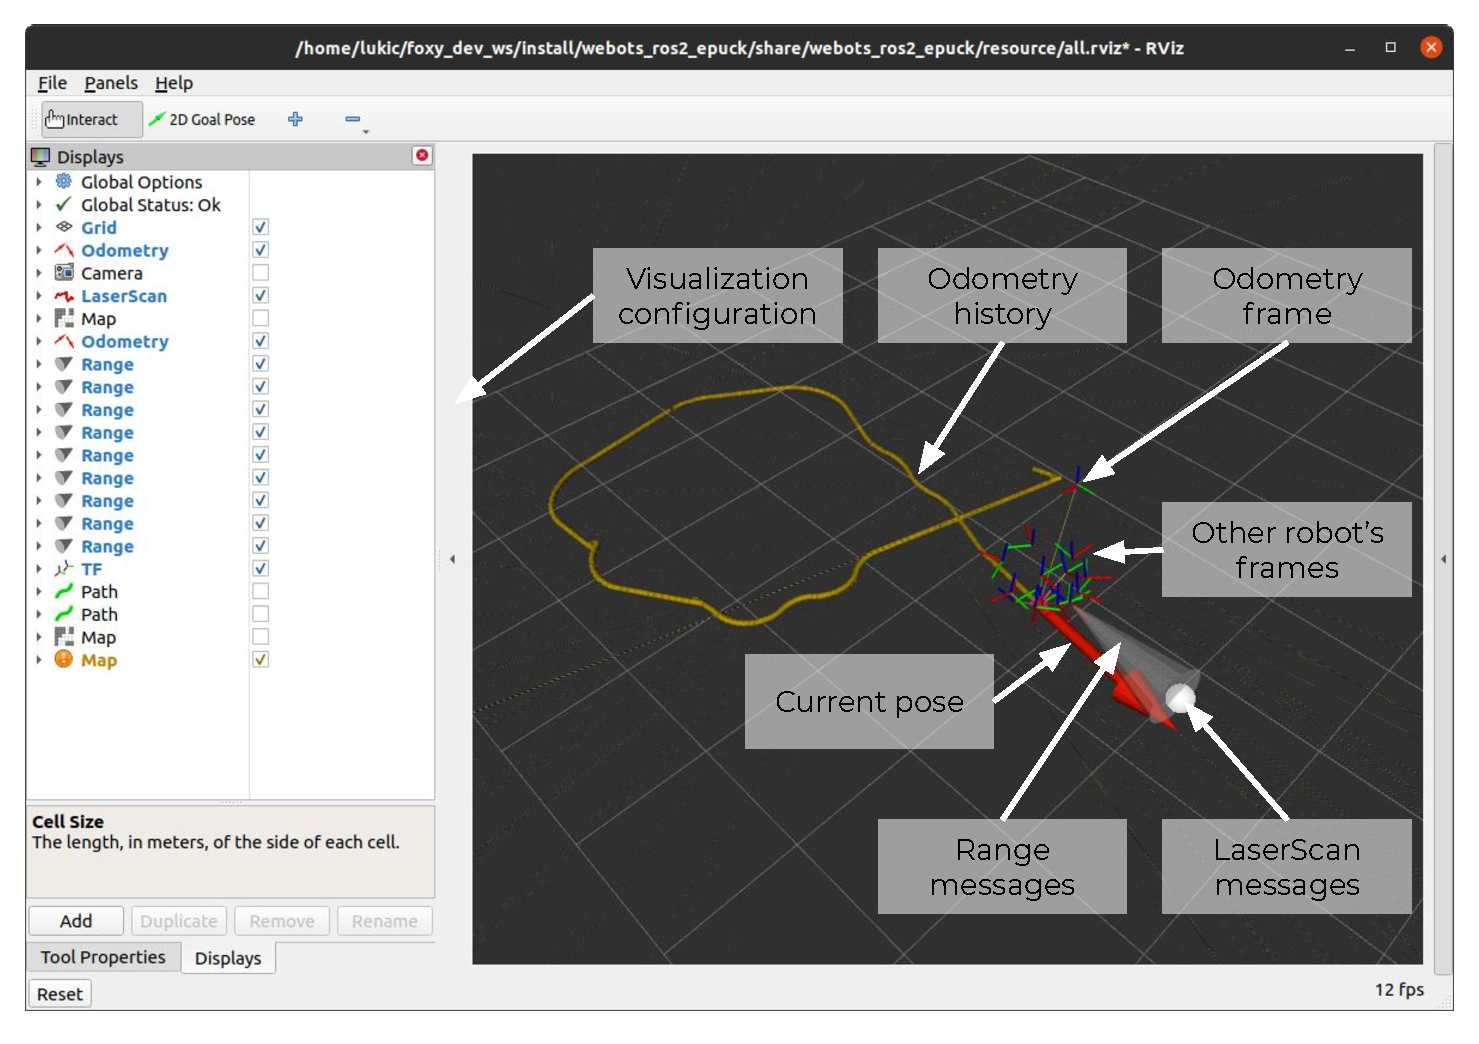
\includegraphics[width=\textwidth]{demos/figures/rviz.pdf}
    \caption{Typical visualization of e-puck2 in \acs{rviz2}}
    \label{fig:demos:rviz}
\end{figure}

\ac{rviz2} is very customizable, meaning it can visualize different aspects of the robot depending on the user's needs.
Once the user is satisfied with the visualization, the view can be saved to a file, for later reuse.
In this master project, there are many \ac{rviz2} configurations provided, optimized for different scenarios like sensor inspection, mapping, and navigation.
These configurations will be automatically loaded, depending on the launch file that is used.

In Figure \ref{fig:demos:rviz} a default view of \acs{rviz2} for the e-puck2 robot is shown.
It visualizes the robot's pose obtained from the odometry, history of odometry readings, different coordinate systems (like odometry, robot's base, distance sensors and similar), range, and laser scan measurements.

\section{Drive Calibration}

Two constants are essential in order to have accurate odometry: wheelbase (distance between the contact points of the two wheels), and wheel radius.
These constants can be measured, but even with the perfect measurements, they are subject to systematic odometry errors, caused by imperfections in the design and mechanical implementation of a mobile robot.
Typical systematic error is uncertainty about the wheelbase and means that the rubber tires contact the floor not in one point, but rather in a contact area \cite{borenstein_measurement_1996}.

Therefore, we use \texttt{/odom} and \texttt{/cmd\_vel} topics that are previously created to calibrate the two important constants for odometry.
The technique is inspired by the one presented in \cite{borenstein_measurement_1996}; the robot should move linearly, we can compare anticipated distance (self-reported distance) with the actual distance.
The linear movements allow us to adjust the wheel radius.
For the wheelbase, the robot is rotated a predefined number of rotations; then, it is compared to the actual number of rotations, and wheelbase is adjusted accordingly (see Figure \ref{fig:demos:diff_drive_calibration}).

\begin{figure}[H]
    \centering
    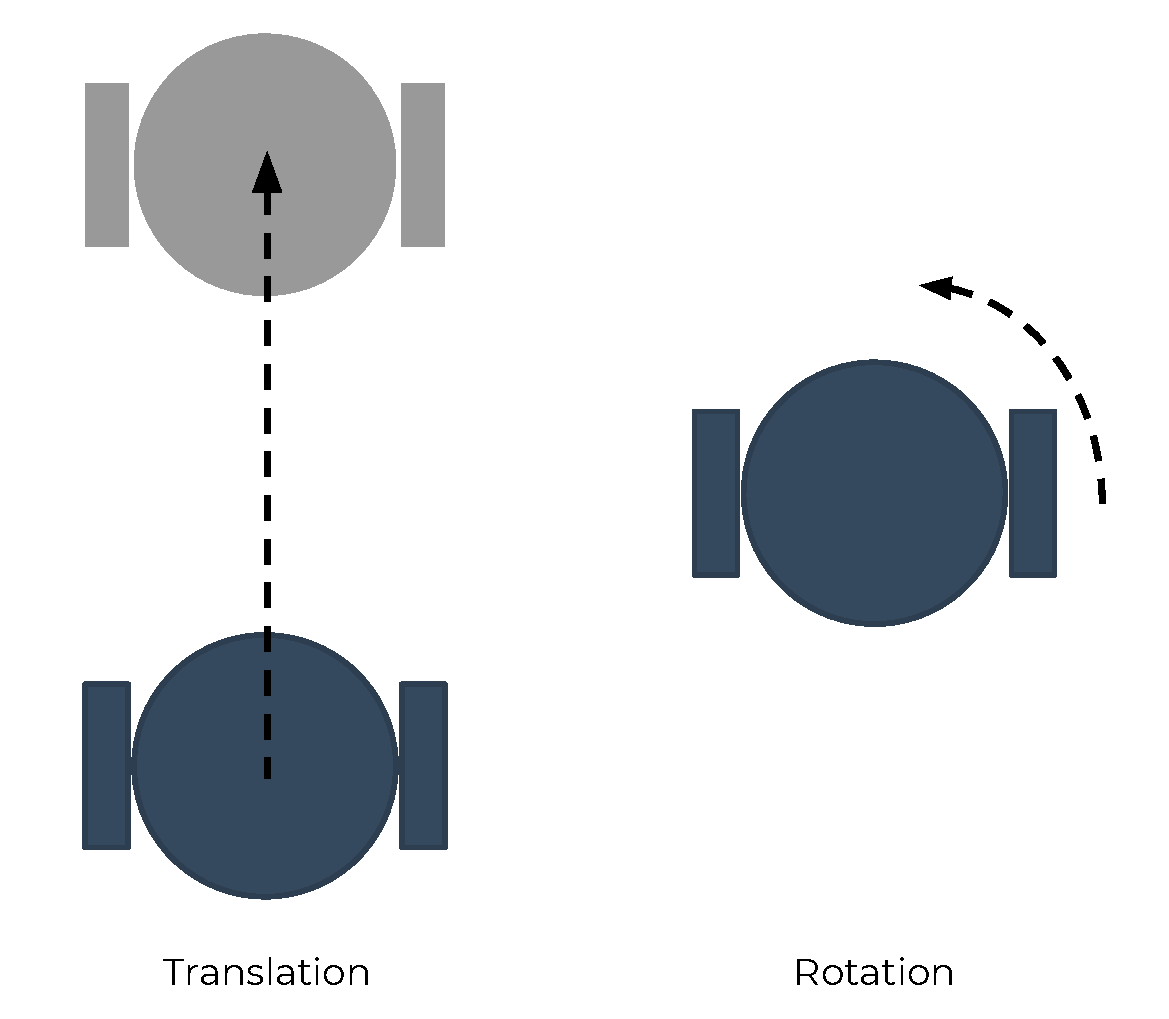
\includegraphics[width=0.7\textwidth]{demos/figures/calibration.pdf}
    \caption{Differential drive robot calibration process}
    \label{fig:demos:diff_drive_calibration}
\end{figure}

The custom-created node continuously receives the readings from the \texttt{/odom} topic to stop the robot exactly when the robot reaches the goal position.
It also sets appropriate linear or angular velocity depending on the type of the test.
Finally, the calibration node is successfully utilized for odometry calibration of the e-puck2 robot.
% Effectively, this node shows that \texttt{/odom} and \texttt{/cmd\_vel} topics are properly implemented while providing a useful feature.

\section{Custom Mapper Node}
\label{sec:demos:mapping}

The goal of the next example is to utilize a larger portion of the created \ac{ros2} interface.
The goal is to map the environment using an e-puck2 robot and its distance sensors.
A few approaches are considered to meet the goal:
\begin{itemize}
    \item Utilize the existing \ac{slam} solutions available for \ac{ros2} (\texttt{slam\_toolbox} or \texttt{cartographer}).
    \item Create a simple custom solution.
    \item Make a bridge to \ac{ros}1 workspace and use \ac{slam} solutions available for \ac{ros}1 (e.g. \texttt{gmapping} is only available for \ac{ros}1).
    \item Port \texttt{gmapping} \ac{slam} solution (that is available only for \ac{ros}1) to \ac{ros2}.
\end{itemize}

In tests, \texttt{slam\_toolbox} and \texttt{cartographer} were not able to provide accurate mapping due to the scarcity of the distance measurements\footnote{The author of \texttt{slam\_toolbox}, Steve Macenski, explained that modern graph-based \ac{slam} solutions do not provide good results when used with e-puck2 robot (or similar robots with a few distance sensors) like old particle filter based \ac{slam} solutions - \url{https://github.com/SteveMacenski/slam_toolbox/issues/192}.}. Using \texttt{gmapping} through \ac{ros}1 bridge indeed gave a good results.
However, complex installation and usage is something we tried to avoid as it is not user-friendly.
Porting \texttt{gmapping} to \ac{ros2} is feasible, but maintenance of a such complex software would be time intensive.

Finally, considering the scope of this master project and the high precision of e-puck2 odometry, the decision was to create a simple mapping node.
The node uses odometry exclusively for localization.
In general, this is not the right solution knowing that the odometry accumulates the error, but it provides satisfying results for small maps. 

\vspace*{.4cm}
\begin{algorithm}[H]
\SetKwInOut{Input}{input}
\SetKwInOut{Output}{output}
\Input{%
    $\bm{L_{scans}}$ -- Laser scan readings \newline 
    $\bm{P_{odom}}$ -- Position of the robot obtained from the odometry
}
\Output{%
    $\bm{M_{map}}$ -- Map of type \texttt{nav\_msgs/OccupancyGrid}
}

$ O_{world} = [\hspace{2mm}] $ \tcp{List of coordinates of obstacles}
use \texttt{tf2} to get position of laser scanner $ P_{scan} $\;

\For{each $ L_{scan} $  in $ L_{scans} $}{
    determine angle of ray ($ \alpha $) from index\;
    $ O_{x} \leftarrow P_{scan} + L_{scan} cos(\alpha) $\;
    $ O_{y} \leftarrow P_{scan} + L_{scan} sin(\alpha) $\;
    add coordinates ($O_{x}$, $O_{y}$) to $ O_{world} $\;
}

write coordinates ($O_{x}$, $O_{y}$) to $ M_{map} $\;
use Bresenham's line algorithm to write empty space\;

\caption{Mapping process}
\label{alg:demos:mapping_process}
\end{algorithm}
\vspace*{.4cm}

The algorithm (see Alg. \ref{alg:demos:mapping_process}) uses a power of \texttt{tf2} package which listens for messages of \texttt{/TfMessage} to determine position of the virtual laser scanner in respect to the odometry frame.
With a few transformations, it is straightforward to calculate the position of the obstacles on the map.
To fill the empty space between the robot and the obstacle (white pixels in Figure \ref{fig:demos:mapping}) Bresenham's line algorithm is implemented \cite{borenstein_measurement_1996}.

\begin{figure}[H]
\centering
\begin{subfigure}{.95\textwidth}
  \centering
  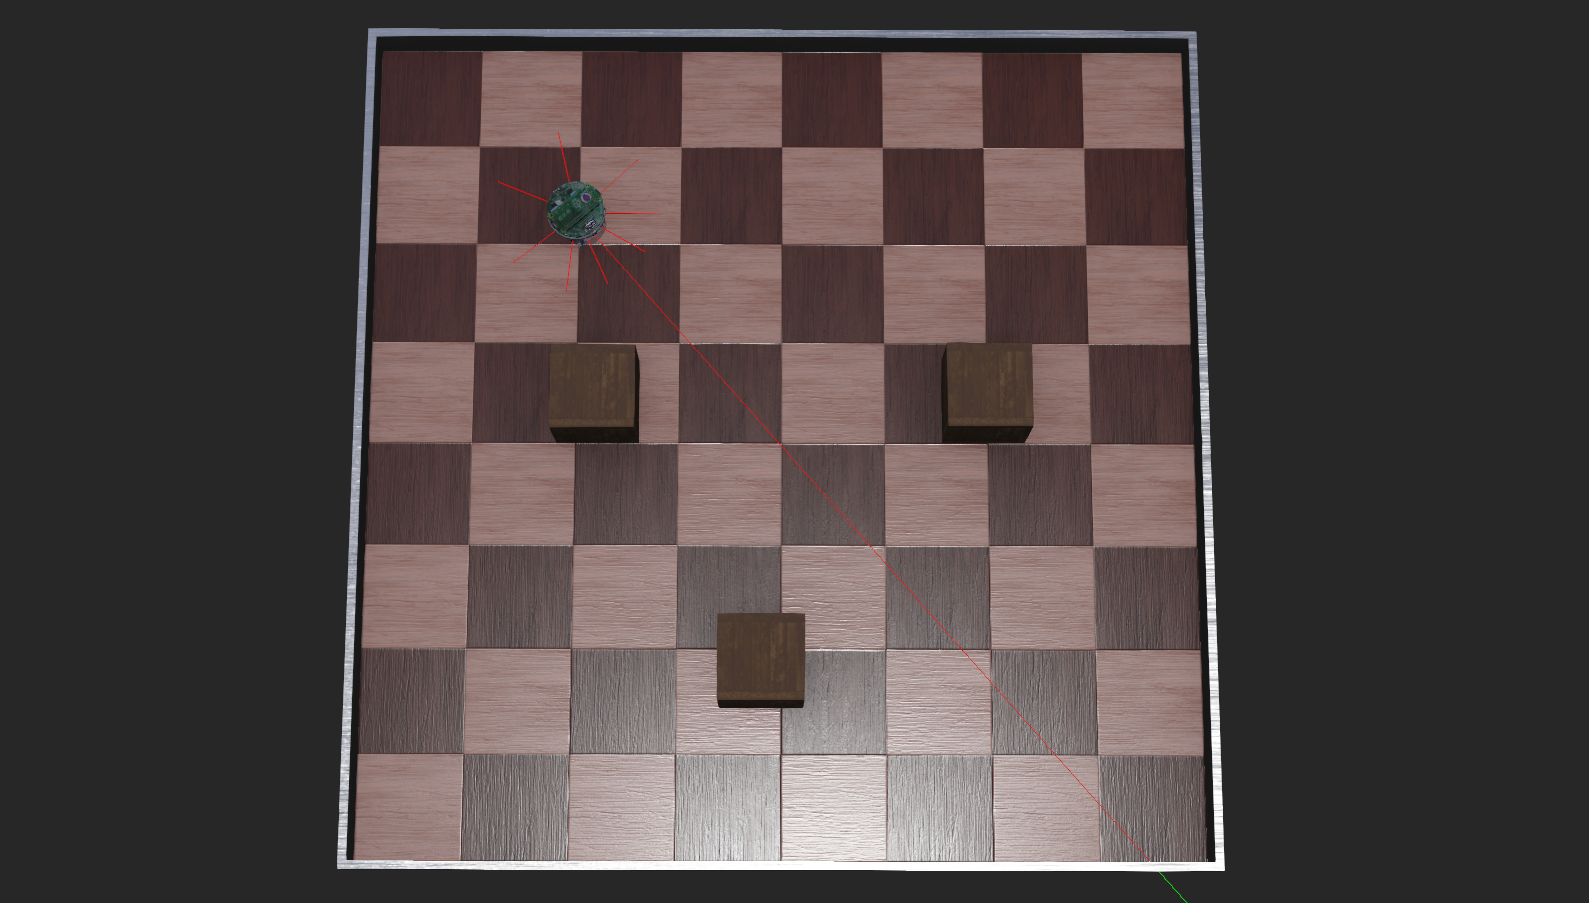
\includegraphics[width=\linewidth]{demos/figures/map_webots.png}
  \caption{Webots simulation with e-puck2}
  \label{fig:demos:mapping:map_webots}
\end{subfigure}
\begin{subfigure}{.95\textwidth}
  \centering
  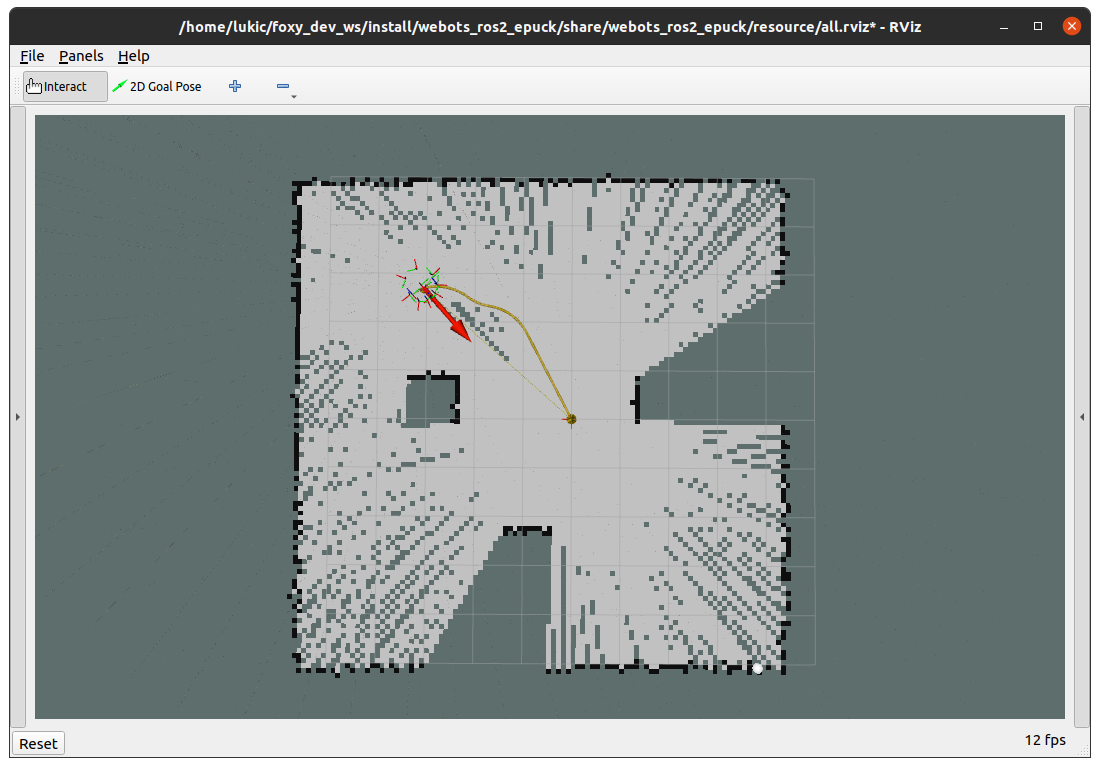
\includegraphics[width=\linewidth]{demos/figures/map_rviz.png}
  \caption{Map visualized in RViz2}
  \label{fig:demos:mapping:map_rviz}
\end{subfigure}
\caption{Mapping results shown in RViz2}
\label{fig:demos:mapping}
\end{figure}

Finally, the result can be observed in the figure above (Figure \ref{fig:demos:mapping}).

\section{Navigation Integration}
\label{sec:demos:navigation}

Another example is navigation.
For this demo, the Navigation2 community package is integrated.  
\begin{figure}[H]
    \centering
    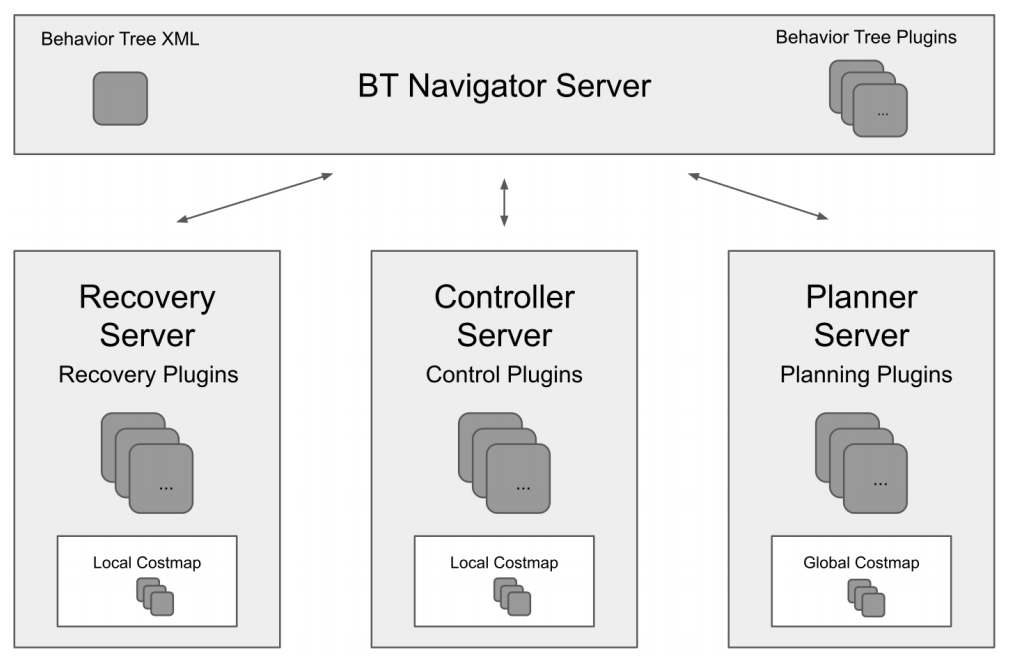
\includegraphics[width=\textwidth]{demos/figures/navigation_overview.png}
    \caption[Architecture of the Navigation2 package]{Architecture of the Navigation2 package\footnotemark}
    \label{fig:demos:navigation_overview}
\end{figure}
\footnotetext{The image is taken from official Navigation2 GitHub repository available at \url{https://github.com/ros-planning/navigation2}.}

% The package is extremely configurable, including hundreds of parameters.
% Therefore, it requires a good understanding of the background theoretical concepts to configure it efficiently \cite{zheng_ros_nodate}.

It uses transforms, maps, and measurements from range finders to control the robot's velocity, effectively avoiding obstacles and converging towards the destination (see Figure \ref{fig:demos:navigation_overview}).
Based on the provided map, it builds a global cost map used by a planner to find a global path (e.g., using an A star algorithm) to the destination.
Based on the data from the range finders, it builds a local cost map that is used by the controller server to avoid obstacles locally.
The controller server is also used to follow the path generated by the planner server, and it usually uses implementation called DWB local planner.
The planner considers the robot's maximum rotational and linear velocity and various critics (e.g., goal align and path align), to issue velocity commands \cite{macenski_marathon_2020-1}. 

% TODO: Add RViz2 screenshot
}{}
\chapter{The Generalization of \ac{ros2} Interface for Webots}
\label{chap:generalization}
\shorttitle{\nameref{chap:generalization}}


\section{Introduction}
\label{sec:generalization:introduction}

Up to now, \ac{ros2} interface for the e-puck2 robot in Webots is created manually.
It means that the Webots controller has to be written to exposes \ac{ros2} interface.
Although this method gives a developer much flexibility, it is time demanding, prone to errors, and requires changes every time the Webots robot model is alternated.
Since the Webots model is accessible from Webots \ac{api}, we saw an opportunity to automate the process of creating \ac{ros2} driver for Webots.

% objectives (hybrid)
The primary objective is to create a universal launch file that is supposed to read the Webots robot model and create \ac{ros2} interface accordingly.
This process has to be fully automated by default, highly configurable, and it has to work in conjunction with the user's custom code.
The universal launch file allows users to bootstrap the project and benefit from reusable blocks quickly, but also it offers a possibility to configure the \ac{ros2} interface and extend the driver if needed.

% pros and cons
This system supposed to bring a few major advantages for the users, the most important of which is development time.
Instead of writing a custom Webots controller, which exposes \ac{ros2} interface for each robot, the process of creating \ac{ros2} interface could be completely avoided reducing development time significantly.
Besides, if the controller written by the user is not implemented properly, every iteration on the model requires changes in the controller.
For example, if \texttt{lookupTable} field of \texttt{DistanceSensor} is changed in model, the controller should be updated accordingly.
The second major advantage of the universal driver is less prone to errors.
Since the universal driver is supposed to be maintained by the Webots team and community, the bugs should be discovered and fixed quickly.
However, the universal driver and launch introduce a level of abstraction hiding implementation details and customization possibilities.
Therefore, the building blocks must be carefully designed to allow a high level of customization if a user needs it.

% challenges
As mentioned, the universal driver needs access to the Webots robot model to generate a proper \ac{ros2} interface.
This will present many challenges.
If Webots robot is not configured to work as Supervisor, many aspects of Webots robot model are hidden.
Therefore, Webots controller \ac{api} has to be extended, the most importantly, the \ac{api} needs to be extended to support allow \ac{ros2} transforms.
The other missing functions in Webots \ac{api} is, for example, access to a lookup table of \texttt{DistanceSensor}.
The access to lookup table is needed because \texttt{sensor\_msgs/Range} topic requires real values to be published instead of raw values.



\section{Design}

In the previous section, the idea of Webots to \ac{ros2} interface generalization is presented, focusing on the objective, advantages, and challenges.
Here, more details on the design will be given. Nevertheless, we need to review the approach that has taken place up to now (see Fig. \ref{fig:generalization:ros2_driver_within_webots}). 

% https://docs.google.com/drawings/d/1hRj3ivxq4uhepWZhiJNc_sa_-RWV9RomA9dyEC2PbiI/edit?usp=sharing
\begin{figure}[H]
    \centering
    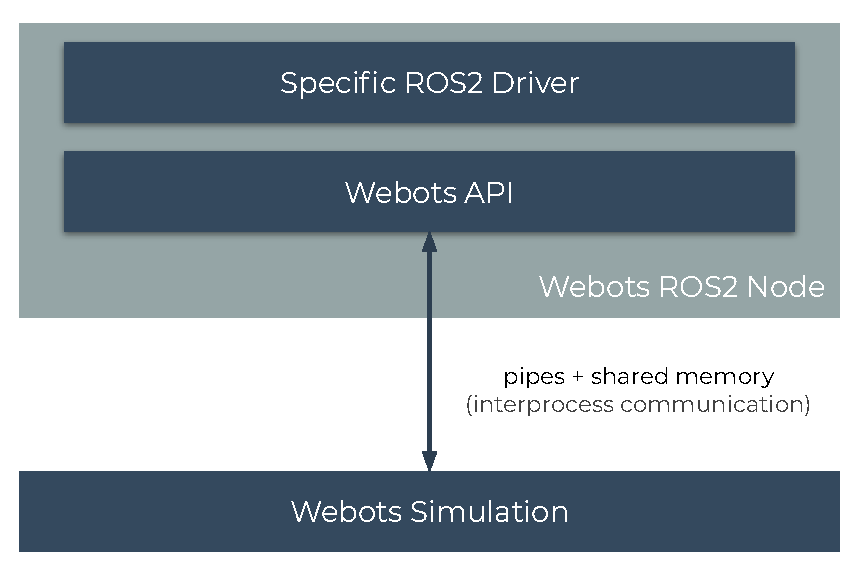
\includegraphics[width=0.8\textwidth]{generalization/figures/ros2_driver_within_webots.pdf}
    \caption{Technique of creating \ac{ros2} interface within Webots before universal driver and launch file are introduced}
    \label{fig:generalization:ros2_driver_within_webots}
\end{figure}

As shown in the picture, the process of creating \ac{ros2} driver required of user to use Webots \ac{api} to write \ac{ros2} driver. 
The user had to write a layer that sits in between low-level \ac{api} (Webots \ac{api} in this case) and \ac{ros2} interface. 
Although this is a necessary step for the real robots and allows users a lot of customization (or even ability to optimize), the objective is to avoid the step as of the reasons given in the previous section (see Section \ref{sec:generalization:introduction}).

Therefore, the new universal driver design is given in the following picture.
\begin{figure}[H]
    \centering
    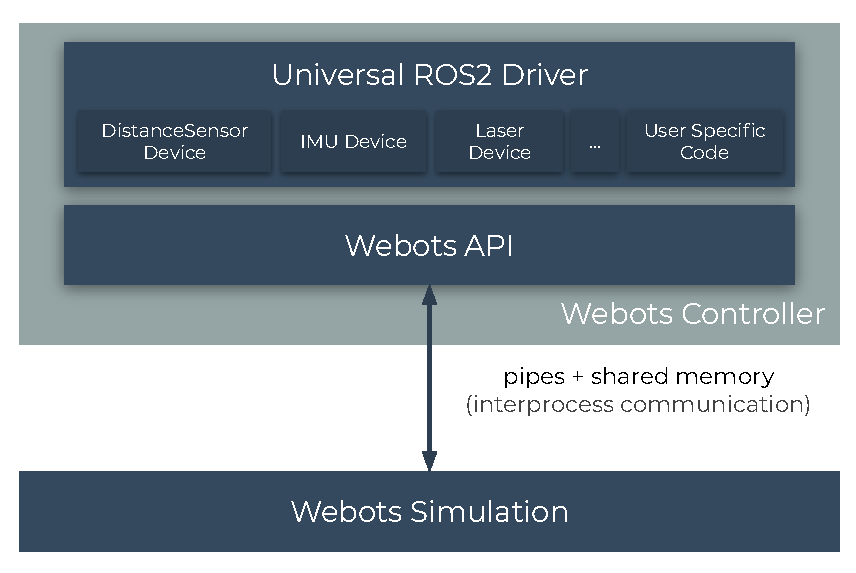
\includegraphics[width=0.8\textwidth]{generalization/figures/universal_driver_within_webots.pdf}
    \caption{Webots and \ac{ros2} interface using the new universal driver}
    \label{fig:generalization:universal_driver_within_webots}
\end{figure}

With the universal driver, a notion of devices is introduced.
A device\footnote{Note that "device" is related to a module in the universal driver and "Webots device" is a node that represents a robot device in Webots}, in this context, represent a module which transforms data from of one or more Webots devices to one or more \ac{ros2} topics and services.
By default, the universal driver will go through all Webots devices available in a robot and try to match them with a suitable device.
If the match is found, a new device is instantiated, a Webots device is assigned to it, and the device will start publishing or subscribing to the \ac{ros2} messages.

All devices are configurable, meaning that it will use default parameters if custom parameters are not supplied.
Since a device can be parameterized from multiple sources, the priority is the following:
\begin{itemize}
    \item A parameter value obtained through \ac{ros2} parameters has the highest priority, and it will override parameter values obtained through any other source.
    \item Python dictionary consisted of parameters passed to the device manager is the second in the priority list.
    \item default or autogenerated values have the least priority. The autogenerated values are usually based on Webots' device names.
\end{itemize}

If a user is not satisfied with the customization achieved by using the parameters, the user can write custom code for it.
A good example is distance sensors in e-puck2.
E-puck2 has nine distance sensors positioned around the robot that could emulate \ac{lidar} and publish data to the \texttt{LaserScan} topic.
Allowing something like this in the universal driver would be too much work, and little gain as the only small number of users would benefit from it.
Therefore, users can disable the ROSification of Webots distance sensors and implement a custom code that will publish measurements to \texttt{LaserScan} topic\footnote{The described example is implemented, explained in more details and it is publicly available.}.

\section{\ac{ros2} Transformations}

In context of \ac{ros2}, transforms represent translation and rotation between two coordinate frames (see Fig. \ref{fig:generalization:tf2_robot}).
Keeping track of the transforms is important as it can provide a relative translation and rotation of two arbitrary coordinate frames in a transforms tree at any point in time \cite{foote_tf_2013}. 
\ac{ros2} considers the transforms as a vital aspect of robotics applications.
Therefore, many \ac{ros2} packages rely on the \ac{ros2} transformations.
For example, \texttt{slam\_toolbox} uses the transforms to find translation and rotation between \texttt{base\_link} and a link that publishes to a topic of type \texttt{LaserScan}.
This is necessary as otherwise, the \texttt{slam\_toolbox} couldn't determine the robot's position in the map.

\begin{figure}[H]
    \centering
    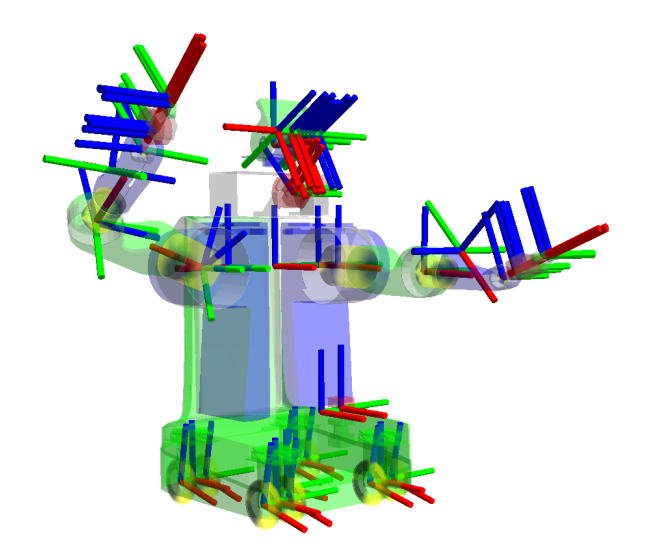
\includegraphics[width=0.8\textwidth]{generalization/figures/tf2_robot.png}
    \caption{An example of coordinate frames visualized in RViz2 \cite{foote_tf_2013}}
    \label{fig:generalization:tf2_robot}
\end{figure}

Considering the importance of transforms \ac{ros2}, the universal driver had to offer functionality to publish those transforms automatically.
To publish transforms automatically, three approaches are considered, two of which are implemented in this project's scope:
\begin{itemize}
    \item Method \#1. The absolute position of each solid node is sampled periodically and published as a dynamic transform. The whole method can be implemented in the universal driver.
    \item Method \#2. A new \ac{api} function is added to Webots, which retrieves a tree of important links and joints. The tree is parsed in the universal driver, and relative transforms are published based on corresponding encoder readings (\texttt{PositionSensor} node in Webots). 
    \item Method \#3. A new \ac{api} function is added to Webots which retrieves \ac{urdf} as a string. \ac{urdf} string is then passed to \texttt{robot\_state\_publisher} as \ac{ros2} parameter. Also, from the universal driver, encoder readings are published periodically as messages of type \texttt{sensor\_msgs/JointState}. These messages are consumed by \texttt{robot\_state\_publisher}, and corresponding transforms are published.
\end{itemize}

The following table compares the most important aspects of these methods.

\begin{table}[H]
    \centering
    \begin{tabular}{|l|c|c|c|}
        \hline
        & Method \#1 & Method \#2 & Method \#3  \\
        \hline
        Preserves noise & No & Yes & Yes \\
        \hline
        Supervisor mode is necessary & Yes & No & No \\
        \hline
        Recognizes static transforms & No & Yes & Yes \\
        \hline
        Implemented in the project scope & No & Yes & Yes \\
        \hline
    \end{tabular}
    \caption{Comparison of different methods considered for publishing \ac{ros2} transforms}
    \label{tab:generalization:transforms_comparison}
\end{table}

As shown in Table \ref{tab:generalization:transforms_comparison}, there are two significant reasons Method \#1 is not used, it does not preserve noise that is coming from the encoders, and the robot has work in supervisor mode.
Even though the implementation does not require introducing changes to Webots core, a considerable disadvantage is a fact that it does not preserve a realistic behavior of the robot supported in Webots.

\subsection{Transforms from \acs{urdf}}
This section describes Method \#3, which is based on exporting an \ac{urdf} document from Webots. 

\subsubsection{\acs{urdf} vs. Webots' Robot Model Representation}
However, it is important to compare \ac{urdf} format and Webots' robot model representation first.
\ac{urdf} is XML format and it uses only two primitives to describe robot model, links and joints.
There has to be at least one link defined in the URDF document, usually named as \texttt{base\_link}, and it's children can be only joints \cite{noauthor_urdf_nodate} (see Fig. \ref{fig:generalization:urdf_vs_webots:urdf}).
Therefore, a link cannot be encapsulated inside another link, but only connected with a common joint.
This is a main difference to Webots' robot representation as the root node in Webots encapsulates other nodes.
In addition to it, Webots has richer specter of nodes.
Besides the links (\texttt{Solid} node in Webots) and joints there are also nodes like \texttt{Group}, \texttt{Transform}, \texttt{Geometry} and \texttt{Shape} (see Fig. \ref{fig:generalization:urdf_vs_webots:urdf}).

\begin{figure}[H]
\centering
\begin{subfigure}{.5\textwidth}
  \centering
  \inputminted{c}{generalization/data/simple.proto}
  \caption{Webots' model representation}
  \label{fig:generalization:urdf_vs_webots:webots}
\end{subfigure}%
\begin{subfigure}{.5\textwidth}
  \centering
  \inputminted[fontsize=\footnotesize]{xml}{generalization/data/simple.urdf}
  \caption{Model representation in \ac{urdf}}
  \label{fig:generalization:urdf_vs_webots:urdf}
\end{subfigure}
\caption{Typical robot representation in \ac{urdf} and in Webots of the same model}
\label{fig:generalization:urdf_vs_webots}
\end{figure}

The described two main differences in a robot model representation, hierarchy and node diversity, make \ac{urdf} export feature implementation rather complicated. 

\subsubsection{\ac{urdf} Export}
\label{subsub:generalization:urdf_export}

In this section, the main points of \ac{urdf} export feature will be described.
It is vital to know that this feature is implemented in Webots core utilizing the existing exporting robot models' mechanisms.
The mechanism already supports a robot model to be exported to \acs{vrml}, \acs{x3d} and PROTO documents.
Even though the mechanism provides useful features, flexibility to implement \ac{urdf} export is limited, and therefore the implementation may differ from what is expected in general (nodes in \ac{urdf} are related by \acs{id}, while nodes in Webots are encapsulated).

The Webots's mechanism to handle exports depends on a few methods declared in \texttt{WbNode}.
In Webots, each node is derived from \texttt{WbNode} class and in the context of \ac{urdf} export it has the following prototype:
\begin{minted}{c++}
class WbNode {
protected:
  // Calls `.writeExport()` to continue the export if needed
  virtual void write(WbVrmlWriter &writer) const;

  // Uses `WbVrmlWriter` to write node details a document
  virtual void writeExport(WbVrmlWriter &writer) const;
  
  // Uses `WbVrmlWriter` to recursively continue export (export children)
  virtual void exportNodeSubNodes(WbVrmlWriter &writer) const;
  
  // Other declarations
};
\end{minted}

Those methods have to be defined for each Webots node to write \ac{urdf} content using \texttt{WbVrmlWriter} class.
Then, the methods are recursively called from the tree root (\texttt{ robot} node) to the leaves.
To export nodes that are related by \acs{id} instead of encapsulating them is shown by the algorithm in Fig. \ref{fig:generalization:urdf_flat}.

\begin{figure}[H]
    \begin{minipage}{\linewidth}
    \begin{procedure}[H]
        \tcc*{$ N_{current} $ and $ N_{queue} $ are global variables. $ N_{current} $ represent a reference on instance of \texttt{WbNode}, while $ N_{queue} $ is a queue of the references}
    
        \If{$ N_{current} \neq $ \texttt{this} $ \land $ \texttt{this} is not joint $ \land $ \texttt{this} is not in $ N_{queue} $}{
            add \texttt{this} to $ N_{queue} $  \;
        }
        
        \If{$ N_{current} $ is not set}{
            $ N_{current} $ = \texttt{this} \;
        }
        
        writeExport(\texttt{this}) \;
        
        \If{$ N_{current} $ = \texttt{this}}{
            \eIf{$ N_{queue} $ not empty}{
                $ N_{current} $ = dequeue the last node from $ N_{queue} $ \;
                write(\texttt{this}, \texttt{writter}) \;
            }{
                $ N_{current} $ = \texttt{NULL} \;
            }
        }
        \caption{write (\texttt{this}, \texttt{writter})}
    \end{procedure}
    \end{minipage}
    \begin{minipage}{\linewidth}
    \begin{procedure}[H]
        \If{$ N_{current} $ = \texttt{this}}{
            write URDF of link \;
        }
        \caption{writeExport (\texttt{this})}
    \end{procedure}
    \end{minipage}
\caption{Approach used to handle \ac{urdf}'s flat nature in object-oriented architecture}
\label{fig:generalization:urdf_flat}
\end{figure}

Properly implementing \texttt{writeExport()} to Webots' nodes that represent joints and links will produce a desired \ac{urdf} document.
However, let consider a very simple example in Fig. \ref{fig:generalization:squashing_transforms:actual}.

\begin{figure}[H]
\centering
\begin{subfigure}{\textwidth}
  \centering
  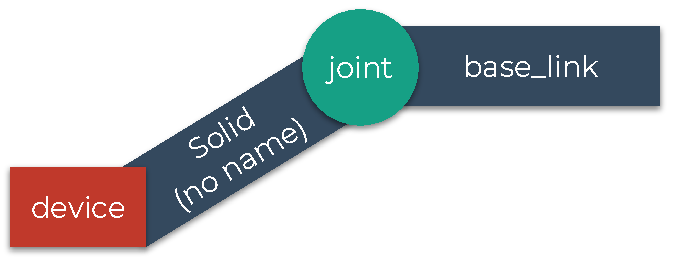
\includegraphics[width=.7\linewidth]{generalization/figures/squashing_transforms_actual.pdf}
  \caption{Exported model}
  \label{fig:generalization:squashing_transforms:actual}
\end{subfigure}
\begin{subfigure}{\textwidth}
  \centering
  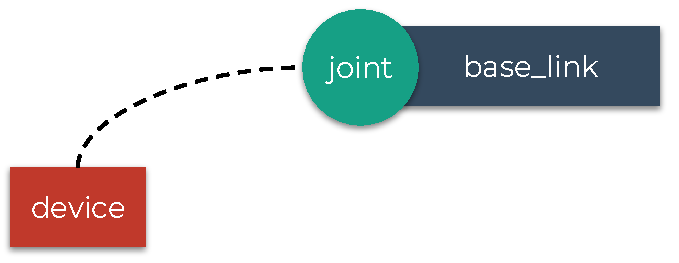
\includegraphics[width=.7\linewidth]{generalization/figures/squashing_transforms_desired.pdf}
  \caption{Webots' model representation}
  \label{fig:generalization:squashing_transforms:desired}
\end{subfigure}
\caption{Typical robot representation in \ac{urdf} and in Webots}
\label{fig:generalization:squashing_transforms}
\end{figure}

In the figure, there is Webots \texttt{Solid} node which got converted to \ac{urdf} link tagged as \texttt{Solid (no name)}. 
Although this may be desirable in some cases, it usually makes \ac{ros2} transform tree complex, which leads to unnecessary computations.
In order to avoid the computations, a squashing is performed.
It means that only relevant Webots nodes are exported into \ac{urdf} (as link nodes) while the others are neglected.
The relevant nodes are all nodes that have \texttt{name} field defined.
Field \texttt{name} is always present for devices, and the user can explicitly define \texttt{name} field if it wants to export as a \ac{urdf} link.

As multiple intermediate Webots nodes can be neglected translation of child node ($I_0$) in respect to it's parent node ($I_N$) is defined as:
\begin{equation}
    \bm{T}_{I_0}^{I_N} = \sum_{i=0}^{N-1} \bm{T}_{I_i}^{I_{i+1}}
\end{equation}
in which translation of intermediate node ($I_m$) in respect to it's parent ($I_n$) is represented $ \bm{T}_{I_m}^{I_n} $ and it is a three-dimensional vector.
Similarly, we do for the rotations:

\begin{equation}
    \bm{R}_{I_0}^{I_N} = \prod_{i=0}^{N-1} \bm{R}_{I_i}^{I_{i+1}}
\end{equation}
Note that $ \bm{R}_{I_0}^{I_N} $ is $ 3 \times 3 $ rotation matrix and matrix multiplication has to be started from the parent.
In the implementation, a node recursively tries to find a relevant parent (visiting nodes towards the tree's root) while adding the visited nodes to the list.
Once the relevant node is reached, it calculates the translation from the first element in the list.

The rotation matrix has to be converted to Euler angles around a fixed axis (extrinsic) roll-pitch-yaw to match \ac{urdf}'s specification. This is done according to \cite[p. 9]{eberly_euler_nodate}.

Finally, the inter-process communication (from Webots simulation to Webots \ac{api}) is extended to support a new function:

\begin{minted}{c}
const char *wb_robot_get_urdf(const char *prefix);
\end{minted}

The \ac{api} function is also exposed to C++, Python, MATLAB, Java and \ac{ros} client libraries.

\subsubsection{Utilization of robot\_state\_publisher}

Once the Webots' \ac{api} is capable of exporting \ac{urdf} as a string it can be utilized in the \ac{ros2} driver to publish \ac{ros2} transforms.
The approach to publish the transform is given in Fig. \ref{fig:generalization:transforms_method_3}.

\begin{figure}[H]
    \centering
    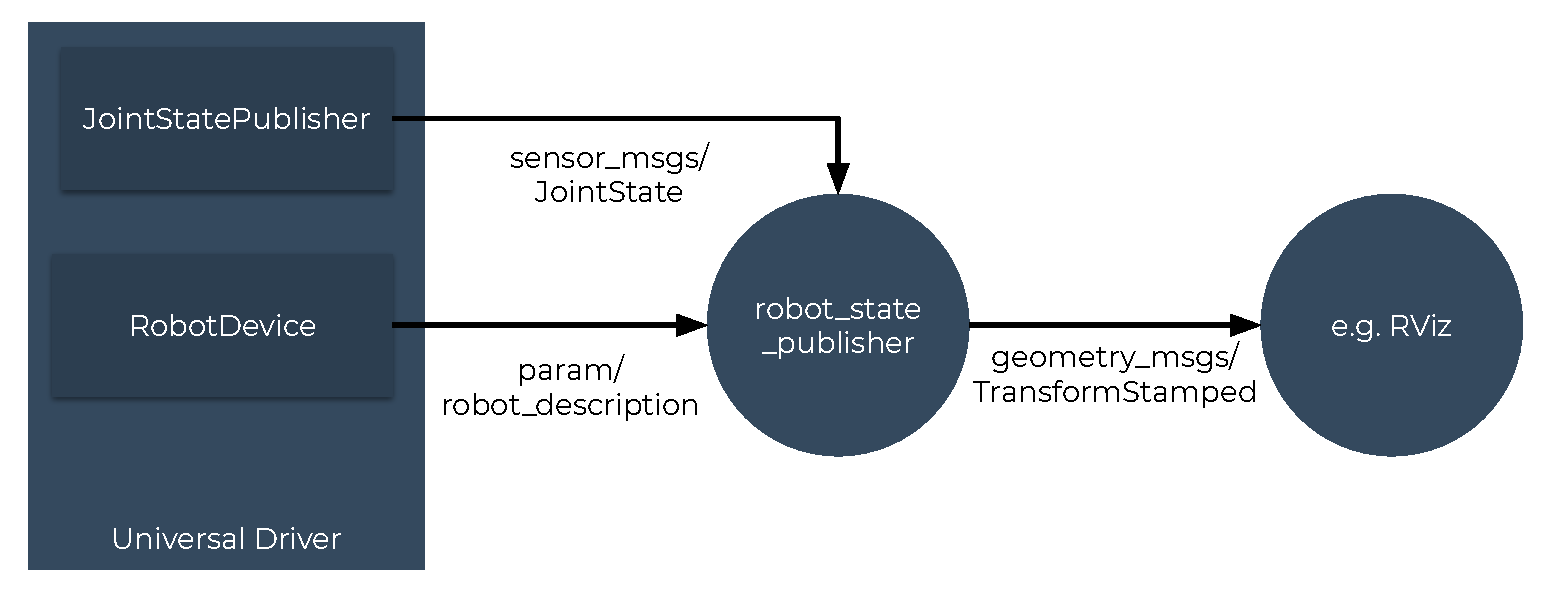
\includegraphics[width=\textwidth]{generalization/figures/transforms_method_3.pdf}
    \caption{Publishing \ac{ros2} transforms using \ac{urdf} and \texttt{robot\_state\_publisher}}
    \label{fig:generalization:transforms_method_3}
\end{figure}

In the figure, the universal driver has to provide parameter \texttt{robot\_description} (\ac{urdf} string) and topic with messages of type \texttt{sensor\_msgs/JointState} which contains readings from Webots \texttt{PositionSensor}s.
The parameter and the topic are consumed by \texttt{robot\_state\_publisher} (\ac{ros2} community node) which publishes \ac{ros2} transformations.

\section{\ac{ros2} Wrapped Devices}
As mentioned before, the universal driver is supposed to create \ac{ros2} automatically interface for each Webots device.
In the master project scope, modules that perform the conversion from Webots to \ac{ros2} interface are created for all Webots devices available on e-puck2, Khepera IV, and TurtleBot3 Burger.
The code is designed to be easily expandable to other Webots devices as well.

In this section, a brief explanation will be given for a few Webots devices.

\subsection{Differential Drive}
The differential drive module interacts with two motors and two position sensors.
The implementation is the same as explained in Section \ref{sec:simulation:odometry_velocity}, but it is decoupled from the rest of the driver to work as an independent component.
Also, it provides a high level of configurability (see table bellow, Table \ref{tab:generalization:diff_driver_params}).

\begin{table}[H]
    \centering
    \begin{tabular}{|l|l|}
        \hline
        \textbf{Name} & \textbf{Description} \\
        \hline
        \texttt{left\_encoder} & Name of position sensor mounted on the left wheel \\
        \hline
        \texttt{right\_encoder} & Name of position sensor mounted on the right wheel \\
        \hline
        \texttt{left\_joint} & Name of motor mounted on the left wheel \\
        \hline
        \texttt{right\_joint} & Name of motor mounted on the right wheel \\
        \hline
        \texttt{wheel\_distance} & Distance between left and right wheel in meters \\
        \hline
        \texttt{wheel\_radius} & Radius of the wheels \\
        \hline
        \texttt{command\_topic} & Topic name on which it should receive velocity commands \\
        \hline
        \texttt{odometry\_topic} & Topic name to which it should publish odometry data \\
        \hline
        \texttt{odometry\_frame} & Odometry frame name used in \ac{ros2} transform messages \\
        \hline
        \texttt{robot\_base\_frame} & Robot base frame name used in \ac{ros2} transform messages \\
        \hline
    \end{tabular}
    \caption{Parameters available for differential drive module}
    \label{tab:generalization:diff_driver_params}
\end{table}

\subsection{Range}
Webots returns value from distance sensors according to specified lookup table\footnote{In the example of lookup table first column represents the actual measurement, the second is the raw measurement, and the third column is the noise}. 

\begin{minted}{python}
lookupTable [ 0     1000  0,
              0.1   200  0.1 ]
\end{minted}

It means it will not necessarily return a real distance to the closest object, but what Webots consider a raw value - linearly interpolated value.
Therefore, to obtain the actual distance, the lookup table has to be read.
The values are then interpolated according to the table.

However, Webots \ac{api} doesn't provide function to retrieve lookup table.
Therefore, the function is implemented\footnote{The \ac{api} function to obtained lookup table is also added for \texttt{Accelerometer}, \texttt{Compass}, \texttt{Gyro}, \texttt{InertialUnit}, \texttt{LightSensor} and \texttt{TouchSensor}.
All \ac{api} functions are also added to C, C++, Python, MATLAB, Java and \ac{ros}.} similarly to one explained in Section \ref{subsub:generalization:urdf_export}.

Then, in the universal controller, the actual values are returned, as shown by the algorithm in Fig. \ref{fig:generalization:interopolation}.

\begin{figure}[H]
    \begin{minipage}{\linewidth}
    \begin{procedure}[H]
        return $ \frac{y_{end} - y_{start}}{x_{end} - x_{start}} (x_{value} - x_{start}) + y_{start}
 $ \;
        \caption{interpolate ($x_{value}$, $x_{start}$, $y_{start}$, $x_{end}$, $y_{end}$)}
    \end{procedure}
    \end{minipage}
    \begin{minipage}{\linewidth}
    \begin{procedure}[H]
        \For{$i\gets0$ \KwTo size of table $ T $ - 1}{
            \If{$(x_{value} T_{raw}[i] \land x_{value} \geq T_{raw}[i + 1]) \lor (
                x_{value} > T_{raw}[i] \land x_{value} \leq T_{raw}[i + 1])$}{
                return interpolate($x_{value}$, $T_{raw}[i]$, $T_{actual}[i]$, $T_{raw}[i+1]$, $T_{actual}[i+1]$) \;
            }
        }

        \tcc*{Extrapolation, assumes the table is sorted in descending order}

        \eIf{$x_{value} > T_{raw}[0] $}{
            return interpolate($x_{value}$, $T_{raw}[0]$, $T_{actual}[0]$, $T_{raw}[1]$, $T_{actual}[1]$) \;
        }{
            return interpolate($x_{value}$, $T_{raw}[-2]$, $T_{actual}[-2]$, $T_{raw}[-1]$, $T_{actual}[-1]$) \;
        }
        \caption{interpolateTable ($x_{value}$, $T$)}
    \end{procedure}
    \end{minipage}
\caption{Procedure used to interpolate table}
\label{fig:generalization:interopolation}
\end{figure}

Once actual values are obtained, the values are packed into messages of type \texttt{sensor\_msgs/Range} and published.

\begin{table}[H]
    \centering
    \begin{tabular}{|l|l|}
        \hline
        \textbf{Name} & \textbf{Description} \\
        \hline
        \texttt{topic\_name} & \ac{ros2} topic name \\
        \hline
        \texttt{timestep} & Publish period in ms  \\
        \hline
        \texttt{disable} & Whether to create \ac{ros2} interface for this sensor \\
        \hline
        \texttt{always\_publish} & Publish even if there are no subscribers \\
        \hline
        \texttt{frame\_id} & Value for \texttt{header.frame\_id} field \\
        \hline
    \end{tabular}
    \caption{Parameters available for distance sensor device}
    \label{tab:generalization:distance_params}
\end{table}

% TODO: \subsection{Camera}
% TODO: \subsection{\ac{lidar}}

\iftoggle{FULL_REPORT}{\chapter{Results and Interpretation}
\label{chap:results}
\shorttitle{\nameref{chap:results}}

\section{Comparison of Physical and Simulated E-puck2}

\subsection{ROS2 Interface for Physical vs Simulated E-puck2}
\subsection{Camera Performance Comparison}
The purpose of this analysis is to determine a suitable way to transport the images from Raspberry Pi Zero and to identify bottlenecks. In the Table \ref{tab:results:camera_perf}, performances are measured in \ac{fps} and the measurements are given for different camera implementations.

\begin{table}[H]
    \begin{adjustwidth}{-1.5in}{-1.5in} 
    \centering
    \begin{tabular}{|c|c|c|c|}
        \hline
         & 32x24 [\ac{fps} ($ \sigma $)] & 160x120 [\ac{fps} ($ \sigma $)] & 640x480 [\ac{fps} ($ \sigma $)] \\
         \hline
         RAW over Wifi & 13.95 (0.009s) & 10.08 (0.013s) & 1.62 (0.096s) \\
         \hline
         RAW on-board & X & X & 3.80 (0.064s) \\
        \hline
        JPEG over Wifi & X & X & 2.97 (0.105s) \\
        \hline
        JPEG over Wifi with white-noise & X & X & 0.95 (0.998s) \\
        \hline
        JPEG on-board & X & X & 2.10 (0.016s) \\
        \hline
        RAW on-board without YUV42RGB & X & X & 5.04 (0.037s) \\
        \hline
        Theora over Wifi & X & X & 1.25 (0.054s) \\
        \hline
        Theora on-board & X & X & 1.03 (0.026s) \\
        \hline
    \end{tabular}
    \end{adjustwidth}
    
    \caption{\ac{fps} measurements in different configurations within \ac{ros2} environment}
    \label{tab:results:camera_perf}
\end{table}

Please note that the experiments are done under the following conditions:
\begin{itemize}
    \item Package \texttt{v4l2\_camera} is used to read and transport images. The package works as following \begin{itemize}
        \item the images are read directly from memory using \texttt{mmap()} in YUV422\_YUY2 format (native camera format),
        \item the images are converted \ac{rgb} using \texttt{cv\_bridge} package and
        \item the images are transported using \texttt{image\_transport}, \texttt{image\_transport\_plugins} (equipped with \texttt{compressed\_image\_transport} and \texttt{theora\_image\_transport}) with default configuration,
        \item the package is alternated to accommodate image resize for this experiment and the image resizing is done just before YUV422\_YUY2 to \ac{rgb} conversion and
        \item the package is implemented in C++ with attention to memory management (the image is cloned only when necessary).
    \end{itemize}
    \item Camera is configured to 15 \ac{fps}.
    \item \ac{fps} measurements are done using \texttt{ros2 topic hz}.
    \item The Wifi network performance measurements are performed using \texttt{iperf3} and the following results acquired: \begin{itemize}
        \item 16.4 Mbits/sec for transfer from PC to Raspberry Pi Zero and
        \item 13.8 Mbits/sec for transfer from Raspberry Pi Zero to PC.
    \end{itemize}
    \item White noise is simulated by putting finger on the camera. The assumption is that the low light condition produces a lot of white noise. 
\end{itemize}

Measured data transfer between Raspberry Pi Zero and PC during the transfer of raw images is 12.8Mb/s which is quite close speed measured using with \texttt{iperf3}. Since every image is sent in \ac{rgb} format that means 7Mb per image ($ 8 \times \frac{ 3 \times 640 \times 480 }{1024 \times 1024}$), or at 1.62 \ac{fps} it is 11.4Mb/s. Therefore, by sending raw images we the most probably encounter limitation of the Wifi network.

\subsection{Performance Comparison in Mapping}
\subsection{Performance Comparison in Navigation}

\section{\ac{ros2} Interface for E-puck2 vs Khepera IV}
\subsection{Performance Comparison in Mapping}
\subsection{Performance Comparison in Navigation}

\section{Benefits of Generalized \ac{ros2} Interface for Webots}
\subsection{Simplification of E-puck2 Driver}
\subsection{Khepera IV Driver Analysis}
\subsection{Going Beyond Khepera IV and E-puck2}
\subsubsection{TurtleBot3 Burger}
\subsubsection{TIAGo}
}{}
\iftoggle{FULL_REPORT}{\chapter{Conclusion and Future Work}
\label{chap:conclusion}
\shorttitle{\nameref{chap:conclusion}}

A \ac{ros2} interfaces are developed for the e-puck2 physical robot and a variety of simulated robots.
A Webots support for \ac{ros2} is improved, providing facilities for automatic creation of a \ac{ros2} interface for various robot models.
The \ac{ros2} interfaces provide a firm abstraction over the robot's simulated and physical hardware. 
Thus, the \ac{ros2} interface allows a \ac{ros2} controller to work with the physical or simulate e-puck2 robot, or with any other simulated robot, without changes needed to the \ac{ros2} controller.
The results prove that researchers can quickly validate their \ac{ros2} controllers on the e-puck2 physical or simulated robot and other Webots simulated robots.
Effectively, closing the loop between the simulation and the physical world.

The thesis summarizes the implementation details of a \ac{ros2} driver for Webots.
It shows how Webots distance sensors, \ac{imu} related sensors, \acp{led}, a camera, motors and encoders are mapped into \ac{ros2} interface.
It introduces how odometry, velocity control, and coordinate frames are generated from basic Webots devices, such as motors and encoders.

The \ac{ros2} driver is also developed for the e-puck2 physical robot, and major challenges in its implementation are given.
It provides a solution to various problems originated from a low-performance computer with an Armv6 architecture. 
Most notably, the tackled challenges are cross-compilation, offloading image compression to \ac{gpu}, unit-testing in \ac{ci} (with x86 architecture), and overall performance issues.

A possibility to automate the creation of \ac{ros2} interface for Webots is observed.
Therefore, a universal \ac{ros2} driver for Webots is developed.
New features are introduced to Webots core to allow automatic creation of the \ac{ros2} interface, most notably \ac{urdf} export.
On top of the Webots, a modular software layer is implemented that performs \ac{api} conversion, from Webots to \ac{ros2}.

The whole project is publicly available on GitHub allowing users and us to further improve it:
\begin{itemize}
    \item Webots to \ac{ros2} conversion layer covers the following Webots nodes: \texttt{Camera}, \texttt{DistanceSensor}, \texttt{Accelerometer}, \texttt{Gyro}, \texttt{InertialUnit}, \texttt{LED}, \texttt{Lidar}, \texttt{LightSensor}, \texttt{Robot}, \texttt{Motor} and \texttt{PositionSensor}. The list of the covered nodes is not exhaustive and more of them should be covered.
    \item \ac{urdf} export does not support visual elements, although the visual elements are useful in RViz2 visualizations. Also, it does not support \texttt{Hinge2Joint}, nor \texttt{BallJoint}.
    \item In certain use-cases pi-puck extension is not necessary and \ac{ros2} could be deployed directly to the \ac{mcu}.
    This will reduce battery usage and overall system complexity, but it will also put limitations such as a dynamic discovering of communication entities within a network.
    \item Additional effort should be put in implementing \ac{ros2} package with \ac{slam} for e-puck2 and similar robots (robots with few distance sensors, that have a very limited range and wide \ac{fov}). 
\end{itemize}
}{}


\cleardoublepage
\addcontentsline{toc}{chapter}{Bibliography}
\bibliography{_references}
\nocite{*}
\bibliographystyle{ieeetr}
%\bibliographystyle{alpha}

\end{document}
